\section{Components of the HPS algorithm : Merging, Splitting and Leaf Computations}
\label{sec:quadtree}
The HPS method applied to \refeq{eq:elliptic_pde} includes a factorization stage and a solve stage. For problems in which for $f(x,y)$ is non-zero, an additional ``upwards'' stage is required for a particular right hand side.  In our algorithm, the build and upwards stages are a recursive application of a 4-to-1 merge algorithm while the solve stage is a recursive application of a 1-to-4 split algorithm.  In this section, we describe these merging and splitting operations.

\ignore{We begin by detailing the computation required on any leaf level patches. We then outline the algorithms for the merging and splitting of families of patches. Next, we demonstrate the HPS method with the build, upwards, and solve stages. }

\subsection{Leaf Level Computations}
\label{sub:leaf_level_computations}

The build stage of the HPS method begins with solving Dirichlet problems at the finest level of a refined quadtree.  Within each quadrant, equation \refeq{eq:elliptic_pde} is discretized on a locally Cartesian mesh.  We refer to this local Cartesian mesh, along with its quadrant as a {\em patch}.  In \reffig{fig:4_to_1_patches} (left), we show four patches in a larger composite domain. The general HPS algorithm does not specify a particular local mesh discretization, and several have been proposed in the literature.  In \citep{gillman2014direct}, the authors use a spectral collocation method and in \citep{fortunato2020ultraspherical}, a Chebyshev tensor product grid for high order finite elements was used. For compatibility with the finite volume code ForestClaw \citep{calhoun2017forestclaw}, we use a second order finite volume discretization of \refeq{eq:elliptic_pde}. Cell-centered finite difference schemes are particularly convenient for adaptively refined Cartesian meshes, since the cell-centered values are not duplicated on adjacent patches.

\begin{figure}
    \centering
    \begin{tabular}{ccc}
        \begin{subfigure}[t]{0.3\textwidth}
            \centering
            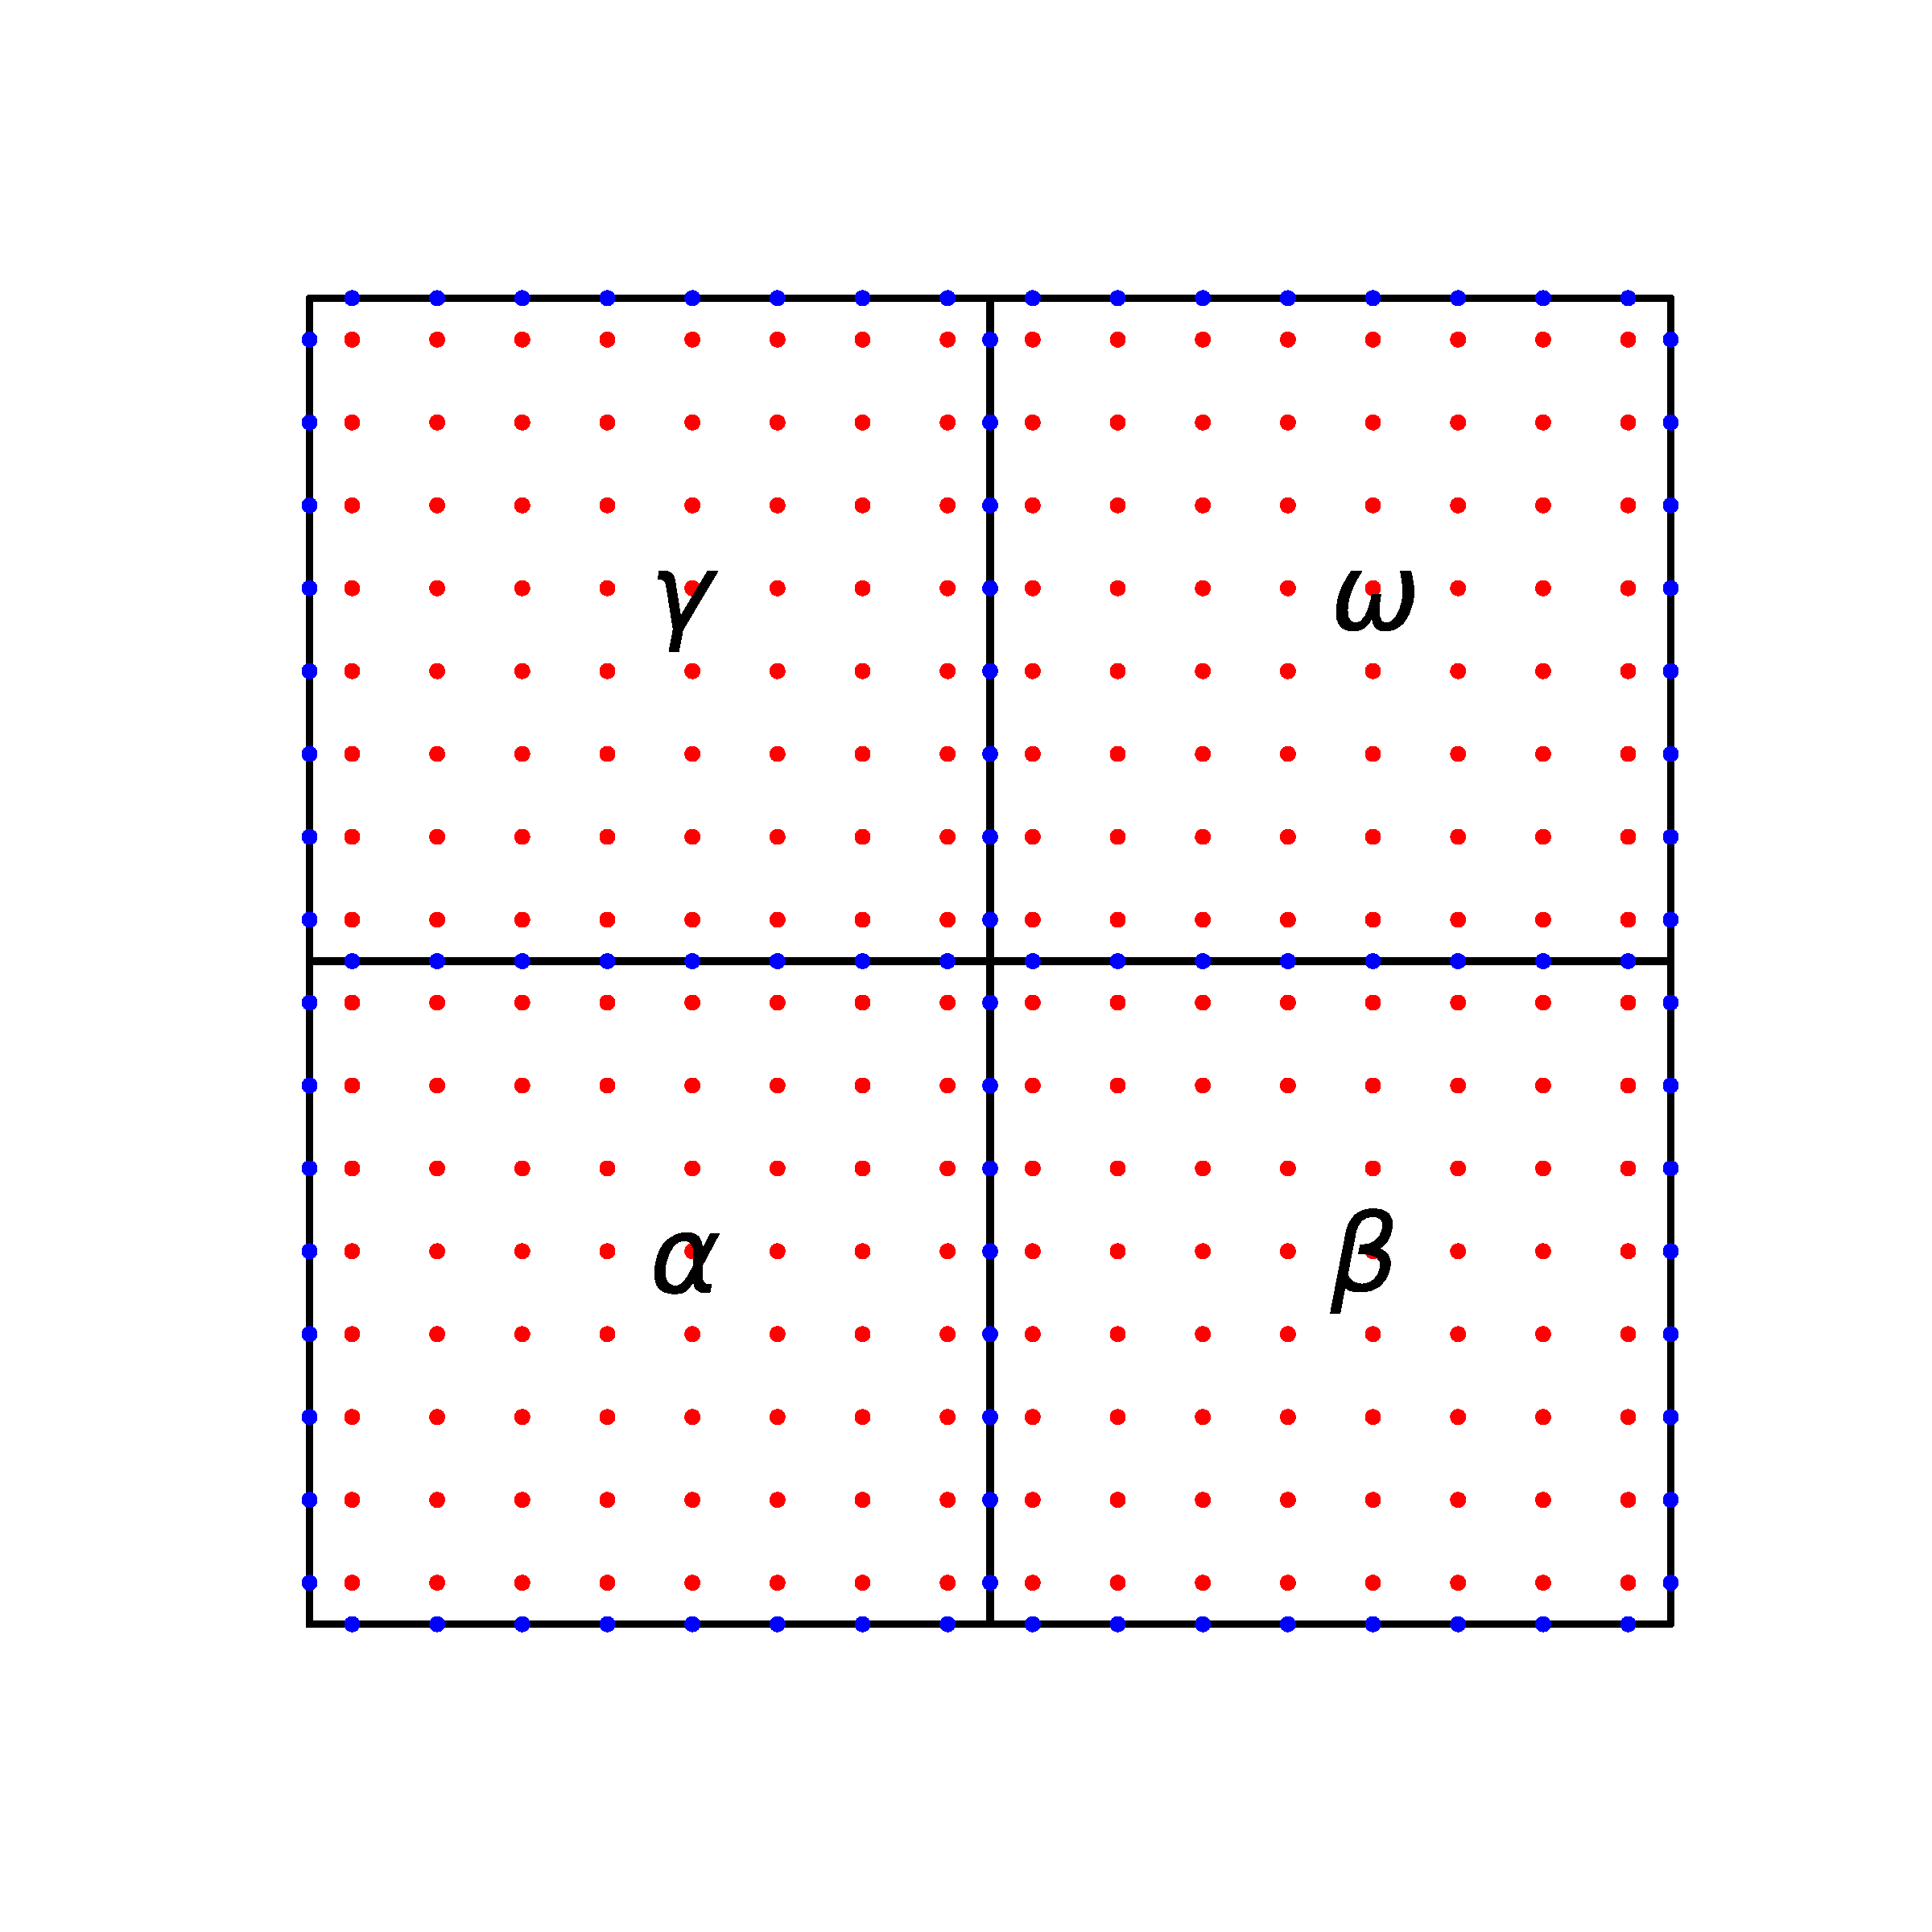
\includegraphics[width=\textwidth, clip=true, trim={100 150 100 150}]{figs/four_patches.pdf}
            \label{subfig:4_patches_with_grid}
        \end{subfigure}
        &
        \begin{subfigure}[t]{0.3\textwidth}
            \centering
            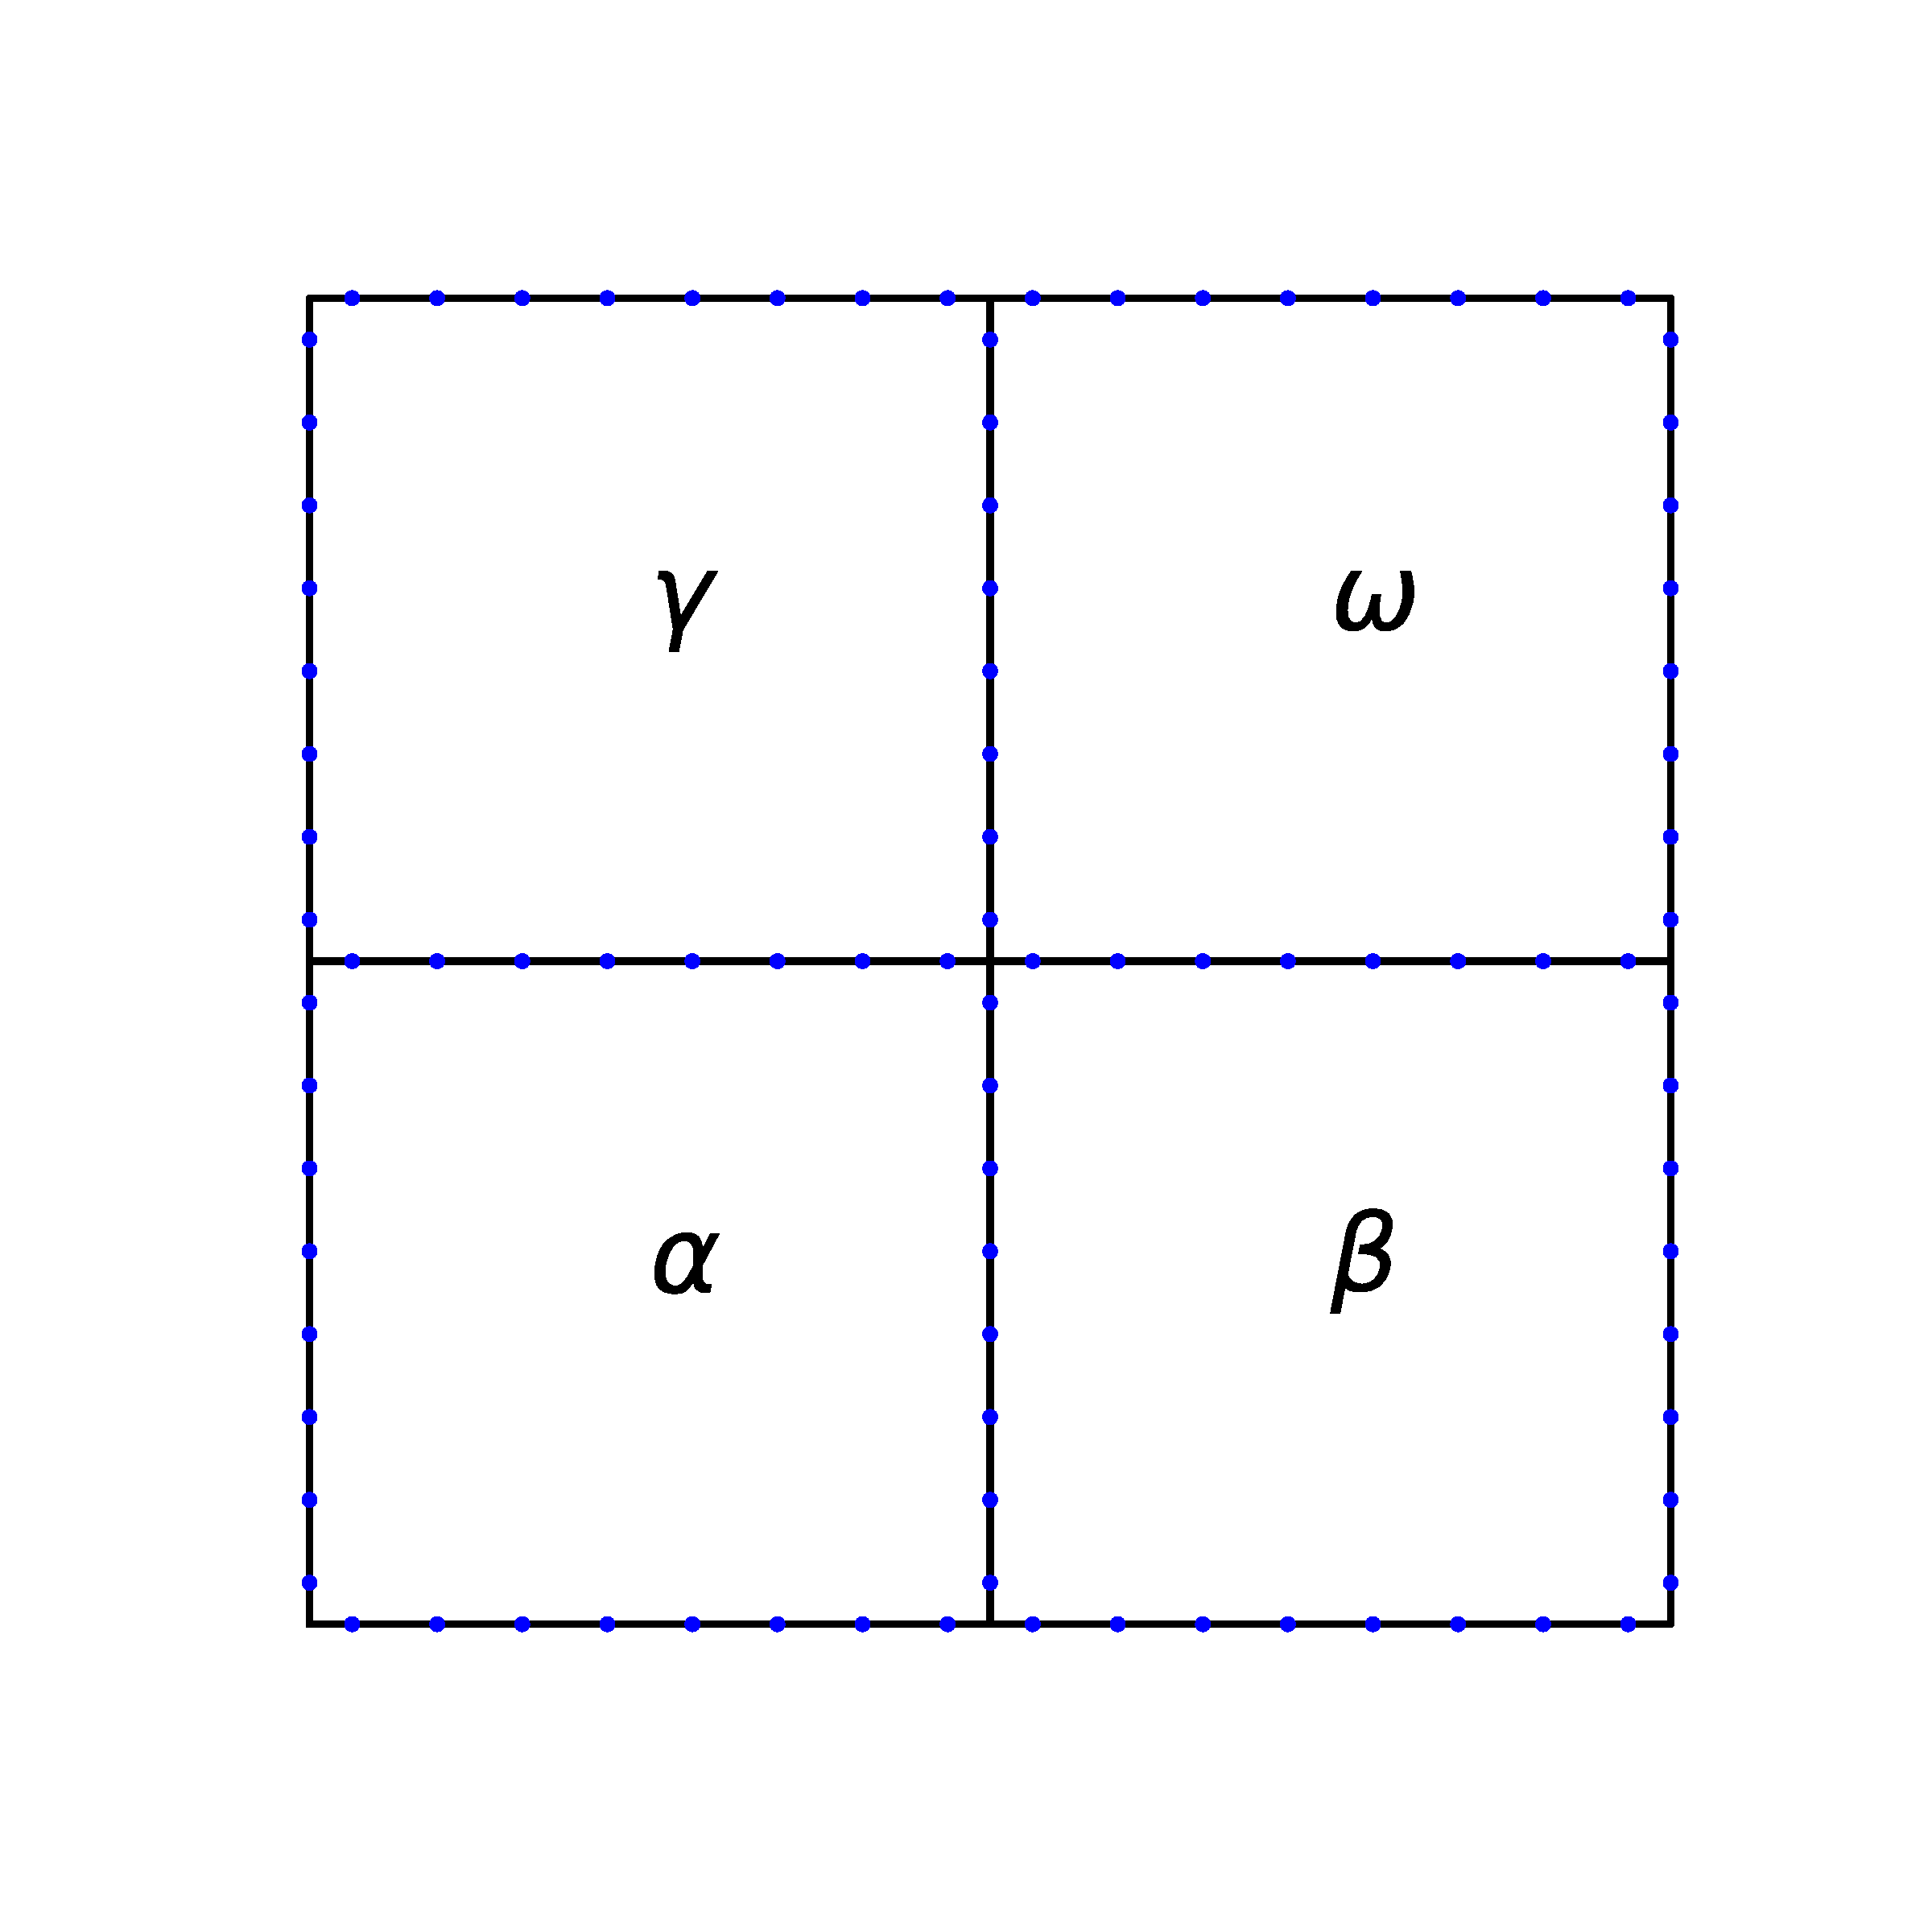
\includegraphics[width=\textwidth, clip=true, trim={100 150 100 150}]{figs/four_patches_without_points.pdf}
            \label{subfig:4_patches}
        \end{subfigure}
        &
        \begin{subfigure}[t]{0.3\textwidth}
            \centering
            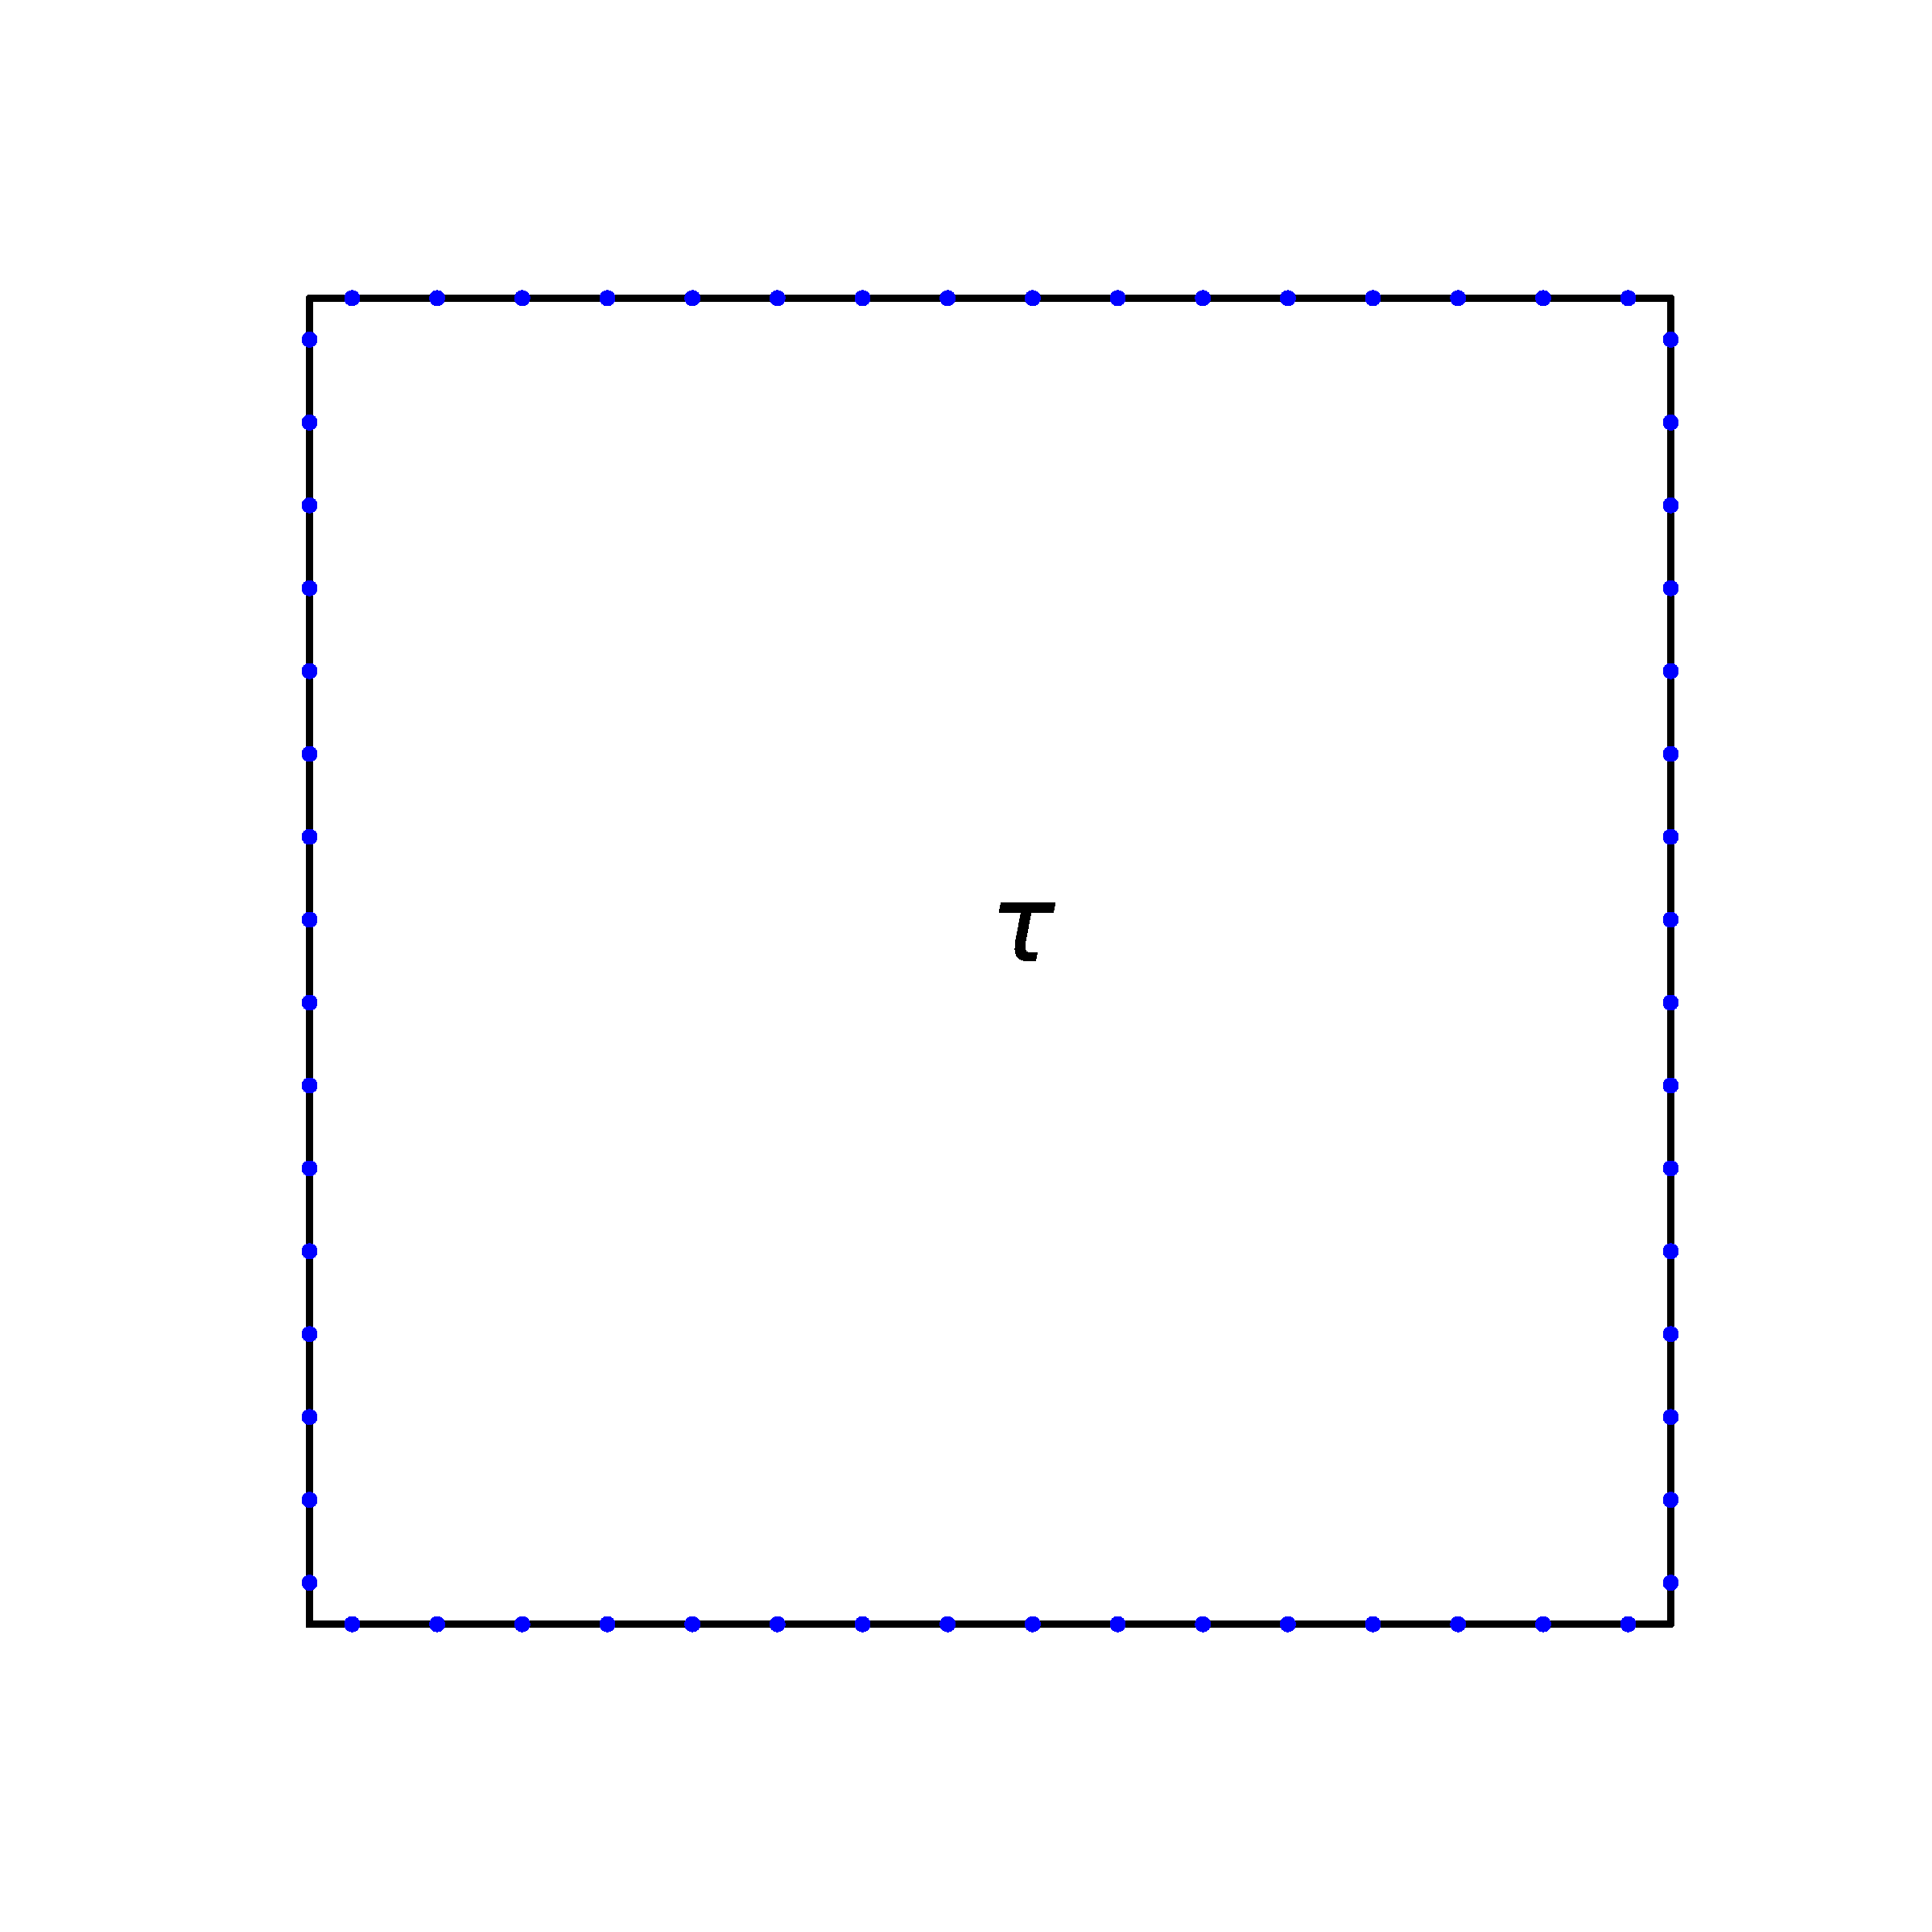
\includegraphics[width=\textwidth, clip=true, trim={100 150 100 150}]{figs/merged_patch.pdf}
            \label{subfig:parent_patch}
        \end{subfigure}
    \end{tabular}
    \caption{The 4-to-1 merge process: (left) the four children patches with their local grid, (middle) the four children share internal and external boundaries with $\tau$, (right) the merged parent patch with data on the exterior of $\tau$.}
    \label{fig:4_to_1_patches}
\end{figure}
Our implementation of the HPS method requires a solver for equation \refeq{eq:elliptic_pde}, subject to Dirichlet boundary conditions, on an $M \times M$uniform Cartesian finite volume grid.   Ideally, this solver uses fast methods, and the value of $M$ should be small enough so the grid fits in CPU cache for optimized cache performance.  A {\em homogeneous} patch solver is one for which the right-hand side data in \eqn{elliptic_pde} is zero.  At the leaf level, we denote the homogeneous patch solver as \Stau and use this solver to map Dirichlet data $\gtau \in \mathcal R^{4M}$ to a grid solution \utau with components $u^\tau_{ij}$, for $i,j = 0,1,2,\hdots M-1$.  Where the context is clear, and accepting some notational abuse,  the operator \Stau can be viewed as matrix of the appropriate size so that $\Stau \gtau = \utau$.  

\ignore{The user or implementor is free to choose a patch solver of their choice. This patch solver takes the role of a matrix operator $\mathbf{S}^{\tau}$ called the solution operator, which maps Dirichlet boundary data to solution data on the interior of the patch. The notation of $\tau$ indicates that $\mathbf{S}$ (and any other matrix operator formed herein) is part of a set, and $\tau$ is the index corresponding to a specific patch.}

A second operator needed at the leaf level is a discrete Dirichlet-to-Neumann (DtN) operator \Ttau that maps Dirichlet data \gtau on the boundary of a patch to Neumann data $\vtau \in \real^{4M}$. Components of boundary data vectors $\gtau$ and $\vtau$ are $g^{\tau}_k$ and $v^{\tau}_k$, $k = 0,1,\hdots 4M-1$, respectively.  To describe our implementation of the Dirichlet to Neumann map, we also assume that we have a discrete cell-centered grid solution $\utau = \Stau \gtau$, with $\utau \in \real^{M^2}$.  The components of the grid solution are given by $u^\tau_{ij}$, $i,j = 0,1,\hdots M-1$.  We define "interior" values $\uin \real^{4M \times 1}$ as those grid solution values \utau for which $i = 0$, $i = M-1$, $j = 0$ or $j = M-1$.  By analogy, components of \uout are grid solution values for which $i=-1$ or $i = M$ or $j = -1$ or $j = M$.   Components of \uin and \uout are $u^{in}_k$ and $u^{out}_k$, respectively.   

Using \uin and \uout, we can discretize the Dirichlet condition as
\begin{equation}
g_k = \frac{u_k^{out} + u_k^{in}}{2}
\end{equation}
Neumann data is discretized analogously as
\begin{equation}
v_k = \frac{u_k^{out} - u_k^{in}}{h}
\end{equation}
Eliminating $u_{k}^{out}$  between the two expressions, we  can express the Neumann data in terms of Dirichlet data and the interior value $u^{in}_k$.  
\begin{equation}
v_k = \frac{2}{h}(g_k - u^{in}_k)
\end{equation}
The vector \vtau can then be expressed as 
\begin{equation}
\vtau = \frac{2}{h}(\gtau - \uin)
\end{equation}

Introducing a matrix $G \in \mathcal R^{4M \times M^2}$ that maps the grid solution \utau to the vector \uin, we write $\uin = G\Stau \gtau$ so that

\begin{equation}
\vtau = \frac{2}{h}(\gtau - G \Stau \gtau) = 
\frac{2}{h}(I - G \Stau)\gtau
\end{equation}
From this, we define the Dirichlet-to-Neumann mapping $\Ttau$ as
\begin{equation}
\Ttau = \frac{2}{h}(I - G\Stau)
\label{eq:map_D2N}
\end{equation}
In practice, we construct \Ttau column-by-column using
\begin{equation}
\mbox{Col}_m(\Ttau) = \frac{2}{h}(I - G \Stau)\mathbf e_{(m)}, \quad m = 0,1,\hdots 4M-1
\end{equation}
where $\mathbf e_{(m)}$ is a $m^{th}$ column of the $4M \times 4M$ identity matrix. 

\ignore{In addition to the solution operator $\mathbf{S}^{\tau}$, a Dirichlet-to-Neumann operator \Ttau is required to be computed at the leaf level. This Dirichlet-to-Neumann (DtN) operator is from a class of operators called Poincaré-Steklov operators that map boundary data from one type to another \citep{quarteroni1991theory}. The DtN operator $\mathbf{T}^{\tau}$ allows neighboring patches to be merged together by equating fluxes across patch boundaries. This allows for a hierarchical merging by recursively eliminating degrees of freedom along patch interfaces -- the core idea of the HPS method.}

\ignore{On each leaf patch, we build operators $\mathbf{S}^{\tau}$ and $\mathbf{T}^{\tau}$, where $\tau$ is the patch index in the composite \pforest mesh. The solution operator $\mathbf S^{\tau}$ solves a boundary value problem (BVP) on the patch subject to Dirichlet boundary conditions on the leaf patch boundary.   For non-leaf nodes of the quadtree, the operator $\mathbf S^{\tau}$ will map Dirichlet data on the node boundary to Dirichlet data to boundaries of children nodes. \ignore{This can be an actual matrix related to $\mathbf{A}^{-1}$ or a function that solves the BVP with the patch discretization and the boundary data. This function is called the {\em patch solver}.} The Dirichlet-to-Neumann (DtN) operator $\mathbf{T}^{\tau}$ is a Poincaré-Steklov operator that maps Dirichlet data specified on the boundary of the patch to Neumann data. The DtN operator is used in the merging of neighboring patches to eliminate degrees of freedom at patch interfaces.}

\ignore{In the original formulation of the HPS method by Gillman and Martinsson \citep{gillman2014direct}, the leaf level operators $\mathbf{S}^{\tau}$ and $\mathbf{T}^{\tau}$ are formed explicitly. By relaxing the requirement of using an explicitly formed solution matrix $\mathbf{S}^{\tau}$ to instead use a function patch solver, the software can be made more general to the discretization on the patches and the solution methodology. In addition, the patch solver function can be used to form the DtN matrix $\mathbf{T}^{\tau}$ without the need to supply it explicitly. \ignore{The generality comes at the cost of optimization for the specific discretization and numerical solver.}}

\ignore{
In this presentation, we use the FISHPACK code as a patch solver, which is based on a cylic-reduction and implemented in the FISHPACK90 library \citep{adams2016fishpack90, swarztrauber1999fishpack,sw-sw:1975}. FISHPACK solves an elliptic PDE using a standard 5-point stencil finite-difference discretization of the elliptic PDE. As a 5-point stencil code, FISHPACK is a second order solver for elliptic PDEs.
}

\ignore{To form the leaf level operators required for the HPS method, assume we have a patch solver described above that can be wrapped in a function called \texttt{PatchSolver}. \texttt{PatchSolver} acts as the matrix operator $\mathbf{S}^{\tau}$ on the leaf level. Furthermore, the function \texttt{PatchSolver} can be used to create a function that performs the action of the DtN operator $\mathbf{T}^{\tau}$. By computing the interior solution via \texttt{PatchSolver} and then computing the discrete derivative along the boundary of the patch, we form a function called \texttt{MapD2N} acts as the matrix operator $\mathbf{T}^{\tau}$. The discrete derivative can be found by a second order extrapolation of the derivative. Finally, the explicit matrix $\mathbf{T}^{\tau}$ can be formed by calling \texttt{MapD2N} for unit potentials along the boundary of a patch to form each column of $\mathbf{T}^{\tau}$. We'll now detail each of these functions and their associated algorithms.}

\ignore{
For a patch of size $M$, let $\mathbf{g}^{\tau} = [\mathbf{g}^{\tau,W}, \mathbf{g}^{\tau,E}, \mathbf{g}^{\tau,S}, \mathbf{g}^{\tau,N}] \in \mathbb{R}^{(4M)}$ be the Dirichlet boundary data and $\mathbf{f}^{\tau} \in \mathbb{R}^{(M \times M)}$ be the RHS data on the interior of a patch $\Omega^{\tau}$. The interior solution data is denoted by $\mathbf{u}^{\tau} \in \mathbb{R}^{(M \times M)}$ and would be computed as $\mathbf{S}^{\tau} \mathbf{g}^{\tau} = \mathbf{u}^{\tau}$. \ignore{, however, we use the aforementioned \texttt{PatchSolver} routine: $\mathbf{u} = $ \texttt{PatchSolver}($\mathbf{g}^{\tau}, \mathbf{f}^{\tau}$).} The Neumann data on the boundary of patch $\Omega^{\tau}$ is denoted by $\mathbf{v}^{\tau}  = [\mathbf{v}^{\tau,W}, \mathbf{v}^{\tau,E}, \mathbf{v}^{\tau,S}, \mathbf{v}^{\tau,N}] \in \mathbb{R}^{(4M)}$. For each side $k$ of the boundary, we compute the discrete Neumann data through a second order stencil involving the Dirichlet data on the boundary and the first interior point from the solution data:
\begin{align}
    v_i^{(k)} = \hat{n}^{(k)} \frac{2}{h} (u_{i,1/2}^{(k)} - g_i^{(k)})
    \label{eq:map_D2N}
\end{align}
where $k = [W, E, S, N]$ is the side index, $i = [0,...,M-1]$ is the index of the point along the side, $M$ is the number of cells per patch side, $\hat{n}$ is the boundary unit normal ($\pm 1$), and $h$ is the grid spacing. The half index on $u$ indicates the first interior point of $u$, or the value of the first interior cell.}

\ignore{
This computation represents the action of the DtN operator $\mathbf{T}^{\tau}$. However, in order to compute the merged solution operators later described, $\mathbf{T}^{\tau}$ needs to be formed explicitly. This can be done by performing the above calculation with a unit potential on the boundary corresponding to a unit vector with a single entry, or $\mathbf{g}^{\tau} = \hat{\mathbf{e}}_j$ with $j = [0,...,4M-1]$. This is done $4M$ times, each corresponding to a column in $\mathbf{T}^{\tau}$ and each point on the boundary of a patch.}

\ignore{This function can be wrapped to create an function that performs the action of $\mathbf{T}^{\tau}$ on Dirichlet data $\mathbf{g}^{\tau}$ to output Neumann data $\mathbf{v}^{\tau}$. This function is called \texttt{MapD2N} and the algorithm is found in \refalg{alg:map_d2n}. Staying consistent with the second order nature of the patch solver, we use a centered difference scheme to compute the unknown Neumann data from the given Dirichlet data and the computed interior solution data.}
\ignore{
\begin{algorithm}
    \caption{\texttt{MapD2N} Function}
    \begin{algorithmic}[0]
        \Require Dirichlet data: $\mathbf{g}^{\tau}$, RHS data: $\mathbf{f}^{\tau}$
        \State $\mathbf{u}^{\tau}$ = \texttt{PatchSolver}($\mathbf{g}^{\tau}$, $\mathbf{f}^{\tau}$) \Comment{Call \texttt{PatchSolver} to obtain interior solution data $\mathbf{u}^{\tau}$}
        \For{$k = 0, \dots, 3$} \Comment{Iterate over sides of patch domain}
            \For{$i = 0, \dots, M-1$} \Comment{Iterate over points on side $k$}
                \State $v_i^{(k)} = \hat{n}^{(k)} \frac{2}{h} (u_i^{(k)} - g_i^{(k)})$ \Comment{$\hat{n}$ is the unit side normal, $h$ is the grid spacing}
            \EndFor
        \EndFor
        \State \Return $\mathbf{v}^{\tau}$
    \end{algorithmic}
    \label{alg:map_d2n}
\end{algorithm}
}  % end ignore

\ignore{While \texttt{MapD2N} performs the action of $\mathbf{T}^{\tau}$ on Dirichlet data $\mathbf{g}^{\tau}$, merging neighboring patches requires an explicit matrix for the DtN operator. To explicity compute $\mathbf{T}^{\tau}$, we solve the boundary value problem with a unit potential at each point on the boundary of the patch to yield a column of the DtN matrix. This is done for each point on the boundary of a patch, and the algorithm is outlined in \refalg{alg:build_d2n}.}

\ignore{
\begin{algorithm}
    \caption{\texttt{BuildD2N} Function}
    \begin{algorithmic}[0]
        \State Initialize $\mathbf{T}^{\tau} = \mathbf{0} \in \mathbb{R}^{[4M \times 4M]}$ \Comment{Create DtN matrix}
        \State Initialize $\hat{\mathbf{e}} = \mathbf{0} \in \mathbb{R}^{[4 M]}$ \Comment{Create vector for unit sources as dummy Dirichlet data}
        \For{$k = 0, \dots, 3$} \Comment{Iterate over sides of patch domain}
            \For{$i = 0, \dots, M-1$} \Comment{Iterate over points on side $k$}
                \State $\hat{e}^{(k)}_i = 1$ \Comment{Set unit source at point on side of patch}
                \State $\mathbf{v} = $ \texttt{MapD2N}($\hat{\mathbf{e}}$, $\mathbf{0}$) \Comment{Solve for Neumann data from unit point source}
                \State $\mathbf{T}^{\tau}[:,i + k M] = \mathbf{v}$ \Comment{Set column of DtN matrix with Neumann data}
                \State $\hat{e}^{(k)}_i = 0$ \Comment{Unset unit source at point on side of patch}
            \EndFor
        \EndFor
        \State \Return $\mathbf{T}^{\tau}$
    \end{algorithmic}
    \label{alg:build_d2n}
\end{algorithm}
} % end ignore

\donna{Move this section?}
\paragraph{Inhomogeneous data} If we have a nonzero right-hand side function $f(x,y)$ in \refeq{eq:elliptic_pde}, a third leaf-level operator is required that maps the inhomogeneous right-hand side data to Neumann data.  We write this mapping as $\Wtau \ftau = \wtau$ and use the mapping $G$ from above to write $\win = G\Wtau \ftau$.  Then the Neumann data is given by 
\begin{equation}
\htau \equiv -\frac{2}{h}\win = -\frac{2}{h}G\Wtau \ftau
\label{eq:htau}
\end{equation}

\ignore{
Finally, for a non-homogeneous elliptic problem, the last leaf level computation necessary prior to merging is to compute the particular data corresponding to the non-homogeneous right-hand side of the PDE. We create a data vector $\htau = [\mathbf{h}^{\tau,W}, \mathbf{h}^{\tau,E}, \mathbf{h}^{\tau,S}, \mathbf{h}^{\tau,N}] \in \real^{(4M)}$ for the particular Neumann data associated with the partition of the BVP. $\mathbf{h}^{\tau}$ is computed by solving the boundary value problem \refeq{eq:elliptic_pde} with zero Dirichlet data, or $\mathbf{g}^{\tau} = 0$, and then mapping it to Neumann data via \refeq{eq:map_D2N}
}

\ignore{calling the \texttt{MapD2N} function with zero Dirichlet data: $\mathbf{h}^{\tau} = $ \texttt{MapD2N}($\mathbf{0}$, $\ftau$).}

\subsection{The 4-to-1 Merge Algorithm}
\label{sub:4-to-1merge}

\donna{Index $\tau$ is being used as a superscript on leaf level computations, i.e. \Stau and \Ttau above. For sibling patches, it makes sense then to use $\alpha$, $\beta$, $\gamma$, $\omega$ as superscripts.}
The goal of the merge process is to merge the Dirichlet-to-Neumann operators associated with four sibling patches into a parent patch operator \Ttau.   We also construct a new solver operator \Stau which maps Dirichlet data on the parent patch to Dirichlet data on each of the four sibling patches.  We denote the children patches as $\alpha$, $\beta$, $\gamma$, and $\omega$ and the merged parent patch as $\tau$ (see \reffig{fig:4_to_1_patches}). Prior to the merge process, each patch will have computed and stored a Dirichlet-to-Neumann matrix \Ti, $i=\alpha, \beta, \gamma, \omega$. \donna{I suggest describing this without referring to index sets, since we are not specifying ordering along the individual edges.}
\ignore{We define an index set intersection between patch $i$ and $j$ as $\mathbf{I}_{ij} = \mathbf{I}_{\partial \Omega_i} \cap \mathbf{I}_{\partial \Omega_j}$ \donna{Define $\Omega_i$ ?}. This is used to form the index sets corresponding to the exterior of the merged patch $\tau$: $\mathbf{I}_{\alpha \tau}$, $\mathbf{I}_{\beta \tau}$, $\mathbf{I}_{\gamma \tau}$, $\mathbf{I}_{\omega \tau}$.} 
\begin{figure}
    \centering
    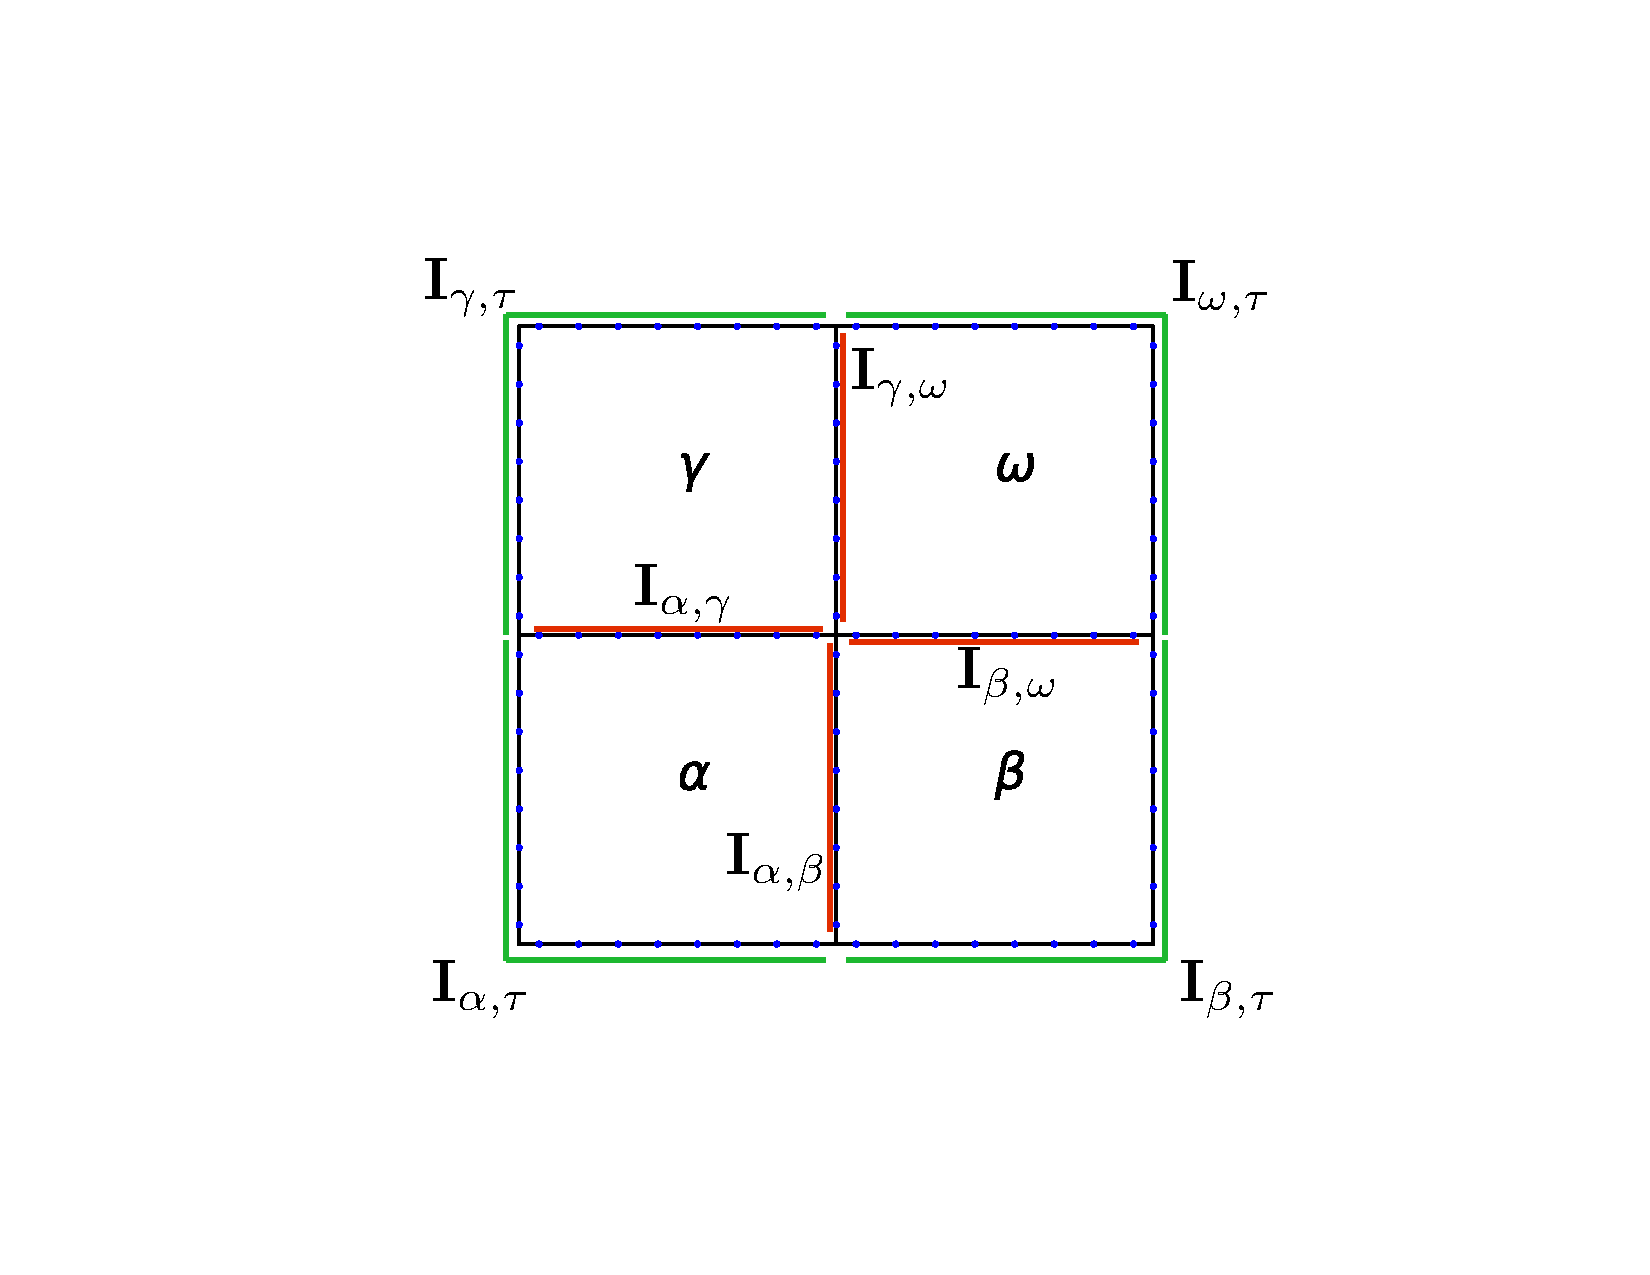
\includegraphics[width=0.5\textwidth]{figs/merging_index_sets.pdf}
    \caption{An overview of the index sets used in the 4-to-1 merge. The index sets marked with green correspond to the exterior of $\tau$ and the index sets marked with red correspond to the interior of $\tau$.}
    \label{fig:merged_index_sets}
\end{figure}

We partition each of the matrices \Ti according to how segments containing Dirichlet data are mapped to segments containing Neumann data.  For example, the sub-matrix $\Talphap{\tau}{\gamma}$ maps Dirichlet data on the boundary shared between sibling patch $\alpha$  and parent patch $\tau$ to the boundary shared between siblings $\alpha$ and $\gamma$.  Following this idea, we partition mappings \Ti as
\begin{equation}
\begin{aligned}
\Talpha \galpha = \valpha \quad & \Longrightarrow  & \quad 
    \begin{bmatrix}
    \Talphap{\tau}{\tau}   &\Talphap{\gamma}{\tau}   & \Talphap{\beta}{\tau} \\
    \Talphap{\tau}{\gamma} &\Talphap{\gamma}{\gamma} & \Talphap{\beta}{\gamma} \\
    \Talphap{\tau}{\beta}  &\Talphap{\gamma}{\beta}  & \Talphap{\beta}{\beta} \\
    \end{bmatrix}
    \begin{bmatrix}
    \galphap{\tau} \\
    \galphap{\gamma} \\
    \galphap{\beta} \\
    \end{bmatrix}
    =
    \begin{bmatrix}
    \valphap{\tau} \\
    \valphap{\gamma} \\
    \valphap{\beta} \\
    \end{bmatrix} \\
&& \\
\Tbeta \gbeta = \vbeta \quad & \Longrightarrow  & \quad
    \begin{bmatrix}
        \Tbetap{\tau}{\tau}   & \Tbetap{\omega}{\tau}   & \Tbetap{\alpha}{\tau} \\
        \Tbetap{\tau}{\omega} & \Tbetap{\omega}{\omega} & \Tbetap{\alpha}{\omega} \\
        \Tbetap{\tau}{\alpha} & \Tbetap{\omega}{\alpha} & \Tbetap{\alpha}{\alpha} \\
    \end{bmatrix}
    \begin{bmatrix}
        \gbetap{\tau} \\
        \gbetap{\omega} \\
        \gbetap{\alpha} \\
    \end{bmatrix}
    =
    \begin{bmatrix}
        \vbetap{\tau} \\
        \vbetap{\omega} \\
        \vbetap{\alpha} \\
    \end{bmatrix} \\
&& \\
\Tgamma \ggamma = \vgamma \quad & \Longrightarrow  & \quad
    \begin{bmatrix}
        \Tgammap{\tau}{\tau}    & \Tgammap{\alpha}{\tau}   & \Tgammap{\omega}{\tau} \\
        \Tgammap{\tau}{\alpha}  & \Tgammap{\alpha}{\alpha} & \Tgammap{\omega}{\alpha} \\
        \Tgammap{\tau}{\omega}  & \Tgammap{\alpha}{\omega} & \Tgammap{\omega}{\omega} \\
    \end{bmatrix}
    \begin{bmatrix}
        \ggammap{\tau} \\
        \ggammap{\alpha} \\
        \ggammap{\omega} \\
    \end{bmatrix}
    =
    \begin{bmatrix}
        \vgammap{\tau} \\
        \vgammap{\alpha} \\
        \vgammap{\omega} \\
    \end{bmatrix} \\
&& \\    
\Tomega \gomega = \vomega \quad & \Longrightarrow  & \quad
    \begin{bmatrix}
        \Tomegap{\tau}{\tau}   & \Tomegap{\beta}{\tau}   & \Tomegap{\gamma}{\tau} \\
        \Tomegap{\tau}{\beta}  & \Tomegap{\beta}{\beta}  & \Tomegap{\gamma}{\beta} \\
        \Tomegap{\tau}{\gamma} & \Tomegap{\beta}{\gamma} & \Tomegap{\gamma}{\gamma} \\
    \end{bmatrix}
    \begin{bmatrix}
        \gomegap{\tau} \\
        \gomegap{\beta} \\
        \gomegap{\gamma} \\
    \end{bmatrix}
    =
    \begin{bmatrix}
        \vomegap{\tau} \\
        \vomegap{\beta} \\
        \vomegap{\gamma} \\
    \end{bmatrix}
\end{aligned}.
\label{eq:linalg_one}
\end{equation}

\ignore{
\begin{align}
    \alpha:
    \begin{bmatrix}
        \mathbf{T}_{\alpha \tau, \alpha \tau} & \mathbf{T}_{\alpha \tau, \alpha \gamma} & \mathbf{T}_{\alpha \tau, \alpha \beta} \\
        \mathbf{T}_{\alpha \gamma, \alpha \tau} & \mathbf{T}_{\alpha \gamma, \alpha \gamma} & \mathbf{T}_{\alpha \gamma, \alpha \beta} \\
        \mathbf{T}_{\alpha \beta, \alpha \tau} & \mathbf{T}_{\alpha \beta, \alpha \gamma} & \mathbf{T}_{\alpha \beta, \alpha \beta} \\
    \end{bmatrix}
    \begin{bmatrix}
        \mathbf{g}_{\alpha \tau} \\
        \mathbf{g}_{\alpha \gamma} \\
        \mathbf{g}_{\alpha \beta} \\
    \end{bmatrix}
    &=
    \begin{bmatrix}
        \mathbf{v}_{\alpha \tau} \\
        \mathbf{v}_{\alpha \gamma} \\
        \mathbf{v}_{\alpha \beta} \\
    \end{bmatrix}
\end{align}
\begin{align}
    \beta:
    \begin{bmatrix}
        \mathbf{T}_{\beta \tau, \beta \tau} & \mathbf{T}_{\beta \tau, \beta \omega} & \mathbf{T}_{\beta \tau, \beta \alpha} \\
        \mathbf{T}_{\beta \omega, \beta \tau} & \mathbf{T}_{\beta \omega, \beta \omega} & \mathbf{T}_{\beta \omega, \beta \alpha} \\
        \mathbf{T}_{\beta \alpha, \beta \tau} & \mathbf{T}_{\beta \alpha, \beta \omega} & \mathbf{T}_{\beta \alpha, \beta \alpha} \\
    \end{bmatrix}
    \begin{bmatrix}
        \mathbf{g}_{\beta \tau} \\
        \mathbf{g}_{\beta \omega} \\
        \mathbf{g}_{\beta \alpha} \\
    \end{bmatrix}
    &=
    \begin{bmatrix}
        \mathbf{v}_{\beta \tau} \\
        \mathbf{v}_{\beta \omega} \\
        \mathbf{v}_{\beta \alpha} \\
    \end{bmatrix}
\end{align}
\begin{align}
    \gamma:
    \begin{bmatrix}
        \mathbf{T}_{\gamma \tau, \gamma \tau} & \mathbf{T}_{\gamma \tau, \gamma \alpha} & \mathbf{T}_{\gamma \tau, \gamma \omega} \\
        \mathbf{T}_{\gamma \alpha, \gamma \tau} & \mathbf{T}_{\gamma \alpha, \gamma \alpha} & \mathbf{T}_{\gamma \alpha, \gamma \omega} \\
        \mathbf{T}_{\gamma \omega, \gamma \tau} & \mathbf{T}_{\gamma \omega, \gamma \alpha} & \mathbf{T}_{\gamma \omega, \gamma \omega} \\
    \end{bmatrix}
    \begin{bmatrix}
        \mathbf{g}_{\gamma \tau} \\
        \mathbf{g}_{\gamma \alpha} \\
        \mathbf{g}_{\gamma \omega} \\
    \end{bmatrix}
    &=
    \begin{bmatrix}
        \mathbf{v}_{\gamma \tau} \\
        \mathbf{v}_{\gamma \alpha} \\
        \mathbf{v}_{\gamma \omega} \\
    \end{bmatrix}
\end{align}
\begin{align}
    \omega:
    \begin{bmatrix}
        \mathbf{T}_{\omega \tau, \omega \tau} & \mathbf{T}_{\omega \tau, \omega \beta} & \mathbf{T}_{\omega \tau, \omega \gamma} \\
        \mathbf{T}_{\omega \beta, \omega \tau} & \mathbf{T}_{\omega \beta, \omega \beta} & \mathbf{T}_{\omega \beta, \omega \gamma} \\
        \mathbf{T}_{\omega \gamma, \omega \tau} & \mathbf{T}_{\omega \gamma, \omega \beta} & \mathbf{T}_{\omega \gamma, \omega \gamma} \\
    \end{bmatrix}
    \begin{bmatrix}
        \mathbf{g}_{\omega \tau} \\
        \mathbf{g}_{\omega \beta} \\
        \mathbf{g}_{\omega \gamma} \\
    \end{bmatrix}
    &=
    \begin{bmatrix}
        \mathbf{v}_{\omega \tau} \\
        \mathbf{v}_{\omega \beta} \\
        \mathbf{v}_{\omega \gamma} \\
    \end{bmatrix}
\end{align}
}

\ignore{The goal is our merge procedure is to obtain $\Ttau$ by {\em merging} $\Ti$ from the four sibling patches. We form the combined system indexed by the exterior and interior of $\tau$ as $\mathbf{I}_{combined} = \{ \mathbf{I}_{ext}, \mathbf{I}_{int} \} = \{ \mathbf{I}_{\alpha \tau}, \mathbf{I}_{\beta \tau}, \mathbf{I}_{\gamma \tau}, \mathbf{I}_{\omega \tau}, \mathbf{I}_{\alpha \gamma}, \mathbf{I}_{\beta \omega}, \mathbf{I}_{\alpha \beta}, \mathbf{I}_{\gamma \omega} \}$. This results in the combined system}

The goal is our merge procedure is to obtain $\Ttau$ by {\em merging} $\Ti$ from the four sibling patches. To do this, we first make the following definitions. 
\begin{equation}
\begin{aligned}
\galphap{\gamma} & = \ggammap{\alpha} \equiv \gzero \\
\gbetap{\omega} & = \gomegap{\beta} \equiv \gone \\
\galphap{\beta} & = \gbetap{\alpha} \equiv \gtwo \\
\ggammap{\omega} & = \gomegap{\gamma} \equiv \gthree \\
\end{aligned}
\end{equation}
Taking the first equation from each of the four sets of equations in \eqn{linalg_one}, we write the first system as
\begin{equation}
A\gext + B \gint = \vext
\end{equation}
where the Dirichlet data has been partitioned into {\em exterior} data and {\em interior} data as
\begin{equation}
\begin{aligned}
\gext & \equiv \left[\galphap{\tau}, \gbetap{\tau} , \ggammap{\tau}, \gomegap{\tau}\right]^T \\
\gint & \equiv \left[\gzero, \gone, \gtwo, \gthree\right]^T \\
\end{aligned}
\end{equation}
The exterior Neumann data is defined as
\begin{equation}
\vext \equiv \left[\valphap{\tau}, \vbetap{\tau} , \vgammap{\tau}, \vomegap{\tau}\right]^T.
\end{equation}
and block matrices $A$ and $B$ are defined as
\begin{equation}
A = \begin{bmatrix}
\Talphap{\tau}{\tau} & \zeromat & \zeromat & \zeromat \\
\zeromat & \Tbetap{\tau}{\tau} & \zeromat & \zeromat  \\
\zeromat & \zeromat & \Tgammap{\tau}{\tau} & \zeromat  \\
\zeromat& \zeromat & \zeromat & \Tomegap{\tau}{\tau} \\
\end{bmatrix}, \qquad
B = \begin{bmatrix}
\Talphap{\gamma}{\tau} & \zeromat              & \Talphap{\beta}{\tau} & \zeromat \\
\zeromat               & \Tbetap{\omega}{\tau} & \Tbetap{\alpha}{\tau} & \zeromat \\
\Tgammap{\alpha}{\tau} & \zeromat              & \zeromat              & \Tgammap{\omega}{\tau} \\
\zeromat               & \Tomegap{\beta}{\tau} & \zeromat              & \Tomegap{\gamma}{\tau}
\end{bmatrix}
\label{eq:matrix_AB}
\end{equation}

To get the second set of equations, we use the equalities between Neumann data at interior boundaries
\begin{equation}
\begin{aligned}
\valphap{\gamma} & = \vgammap{\alpha} \\
\vbetap{\omega} & = \vomegap{\beta} \\
\valphap{\beta} & = \vbetap{\alpha} \\
\vgammap{\omega} & = \vomegap{\gamma}.
\end{aligned}
\end{equation}
to organize the remaining eight equations in \eqn{linalg_one} into four pairs of equations.  These four equations are written as
\begin{equation}
C\mathbf g_{ext} + D\mathbf g_{int} = \zeromat
\end{equation}
where
\begin{equation}
C = 
\begin{bmatrix}
\Talphap{\tau}{\gamma} & \zeromat               & -\Tgammap{\tau}{\alpha} & \zeromat \\
\zeromat               & \Tbetap{\tau}{\omega}  & \zeromat                & -\Tomegap{\tau}{\beta} \\ 
\Talphap{\tau}{\beta}  & -\Tbetap{\tau}{\alpha} & \zeromat                & \zeromat \\
\zeromat               & \zeromat               & \Tgammap{\tau}{\omega}  & -\Tomegap{\tau}{\gamma}
\end{bmatrix}
\end{equation}
and
\begin{equation}
D = \begin{bmatrix}
\Talphap{\gamma}{\gamma} - \Tgammap{\alpha}{\alpha} 
& \zeromat 
& \Talphap{\beta}{\gamma} 
& -\Tgammap{\omega}{\alpha} \\
% 
\zeromat 
& \Tbetap{\omega}{\omega} - \Tomegap{\beta}{\beta} 
& \Tbetap{\alpha}{\omega} 
& -\Tomegap{\gamma}{\beta} \\
% 
\Talphap{\gamma}{\beta} 
& -\Tbetap{\omega}{\alpha} 
& \Talphap{\beta}{\beta}- \Tbetap{\alpha}{\alpha} 
& \zeromat \\
% 
\Tgammap{\alpha}{\omega} 
& -\Tomegap{\beta}{\gamma} 
& \zeromat 
& \Tgammap{\omega}{\omega} - \Tomegap{\gamma}{\gamma}
\end{bmatrix}
\label{eq:matrix_CD}
\end{equation}
\ignore{
form two sets of equations from theTo form the combined system indexed by the exterior and interior of $\tau$ as $\mathbf{I}_{combined} = \{ \mathbf{I}_{ext}, \mathbf{I}_{int} \} = \{ \mathbf{I}_{\alpha \tau}, \mathbf{I}_{\beta \tau}, \mathbf{I}_{\gamma \tau}, \mathbf{I}_{\omega \tau}, \mathbf{I}_{\alpha \gamma}, \mathbf{I}_{\beta \omega}, \mathbf{I}_{\alpha \beta}, \mathbf{I}_{\gamma \omega} \}$. This results in the combined system

\begin{align}
    \mathbf{M} \mathbf{g}_{combined} &= \mathbf{v}_{combined}
    \label{eq:combined_system}
\end{align}
} % end ignore

\ignore{
\begin{align}
    \begin{bmatrix}
        \mathbf{A} & \mathbf{B} \\
        \mathbf{C} & \mathbf{D} \\
    \end{bmatrix}
    \begin{bmatrix}
        \mathbf{g}_{ext} \\
        \mathbf{g}_{int} \\
    \end{bmatrix}
    &=
    \begin{bmatrix}
        \mathbf{v}_{ext} \\
        \mathbf{0} \\
    \end{bmatrix}
    \label{eq:combined_system_matrices}
\end{align}
where
\begin{align}
    \mathbf{A} &= 
    \begin{bmatrix}
        \Talphap{\tau}{\tau} & \zeromat            & \zeromat             & \zeromat \\
        \zeromat             & \Tbetap{\tau}{\tau} & \zeromat             & \zeromat \\
        \zeromat             & \zeromat            & \Tgammap{\tau}{\tau} & \zeromat \\
        \zeromat             & \zeromat            & \zeromat             & \Tomegap{\tau}{\tau}  \\
    \end{bmatrix}
    \label{eq:matrix_A}
\end{align}
\begin{align}
    \mathbf{B} &= 
    \begin{bmatrix}
        \Talphap{\tau}{\gamma} & \zeromat             & \Talphap{\tau}{\beta} & \zeromat \\
        \zeromat               & \Tbetap{\tau}{\omega} & \Tbetap{\tau}{\alpha} & \zeromat \\
        \Tgammap{\tau}{\alpha} & \zeromat             & \zeromat & \Tgammap{\tau}{\omega} \\
        \zeromat               & \Tomegap{\tau}{\beta} & \zeromat & \Tomegap{\tau}{\gamma}
    \end{bmatrix}
    \label{eq:matrix_B}
\end{align}
\begin{align}
    \mathbf{C} &=
    \begin{bmatrix}
        \Talphap{\gamma}{\tau} & \zeromat & -\Tgammap{\alpha}{\tau} & \zeromat \\
        \zeromat & \Tbetap{\omega}{\tau} & \zeromat & -\Tomegap{\beta}{\tau} \\
        \Talphap{\beta}{\tau} & -\Tbetap{\alpha}{\tau} & \zeromat & \zeromat \\
        \zeromat & \zeromat & \Tgammap{\omega}{\tau} & -\Tomegap{\gamma}{\tau}
    \end{bmatrix}
    \label{eq:matrix_C}
\end{align}
\begin{align}
    \mathbf{D} &=
    \begin{bmatrix}
        \Talphap{\gamma}{\gamma} - \Tgammap{\alpha}{\alpha} & \zeromat 
             & \Talphap{\gamma}{\beta} & -\Tgammap{\alpha}{\omega} \\
        \zeromat & \Tbetap{\omega}{\omega} - \Tomegap{\beta}{\beta} & 
            \Tbetap{\omega}{\alpha} & -\Tomegap{\beta}{\gamma} \\
        \Talphap{\beta}{\gamma} & -\Tbetap{\alpha}{\omega} & \Talphap{\beta}{\beta} -  
            \Tbetap{\alpha}{\alpha} &\zeromat \\
        \Tgammap{\omega}{\alpha} & -\Tomegap{\gamma}{\beta} & 
            \zeromat &\Tgammap{\omega}{\omega} - \Tomegap{\gamma}{\gamma} \\
    \end{bmatrix}
    \label{eq:matrix_D}
\end{align}
} % end ignore
\ignore{
In the merge process, we eliminate the points on the interior of $\tau$. To do this, we take the Schur complement of the combined system \eqn{combined_system_matrices}. 
}
Our goal now is to express an operator $\Ttau$ that will map $\mathbf g_{ext}$ to $\mathbf v_{ext}$.  We apply one step of Gaussian elimination to a block augmented system to get
\begin{equation}
\begin{bmatrix}
A & B & \vext\\
C & D & \zeromat\\
\end{bmatrix} 
\quad
\Longrightarrow 
\quad
\begin{bmatrix}
A - BD^{-1}C & 0 & \vext\\
D^{-1}C      & I & \zeromat.
\end{bmatrix}
\end{equation}
or
\begin{equation}
\begin{aligned}
(A - BD^{-1}C) \gext & = \vext \\
\gint & = (-D^{-1} C) \gext.
\end{aligned}
\end{equation}
If we have a non-zero right hand side in \eqn{elliptic_pde}, we must update.  To do this, we define vector \hext as
\begin{equation}
\hext \equiv \left[\halphap{\tau}, \hbetap{\tau} , \hgammap{\tau}, \homegap{\tau}\right]^T 
\end{equation}
where the components have been computed at the leaf level as $\htau = \Rtau \ftau$, above.   We can now write a complete set of equations
\begin{equation}
\begin{aligned}
A\gext + B\gint + \hext = & \vext \\
C\gext + D\gint + \Deltah & = \zeromat
\end{aligned}
\end{equation}
where
\begin{equation}
\Deltah = 
\begin{bmatrix}
\halphap{\gamma} - \hgammap{\alpha} \\
\hbetap{\omega} - \homegap{\beta} \\
\halphap{\beta} - \hbetap{\alpha} \\
\hgammap{\omega} - \homegap{\gamma}
\end{bmatrix}
\end{equation}
From this, we define the merged operators
\begin{align}
    \Xtau & \equiv -\mathbf{D}^{-1} \label{eqs:merged_operators_X} \\
    \Stau & \equiv -\mathbf{D}^{-1} \mathbf{C}  = \Xtau \mathbf{C}
    \label{eqs:merged_operators_S}\\
    \Ttau & \equiv \mathbf{A} - \mathbf{B} \mathbf{D}^{-1} \mathbf{C} 
    \label{eqs:merged_operators_T}
\end{align}
\donna{Minus sign on \Stau?} 
The leaf-level components \hext computed in \eqn{htau} are updated as
\begin{equation}
\hext := \hext - B\Xtau\Deltah
\end{equation}


\begin{remark}
\donna{It is good to point out that indices will have to be re-arranged. But since we don't specify how indices are ordered within each set, it might not be so useful to discuss how the sets are organized.} 

\ignore{If the user is maintaining a specific ordering for the points on the boundary of the patches, then an additional step is necessary after a merge. Computing \Stau and \Ttau in this manner yields matrices that are ordered according to $\mathbf{I}_{combined}$. In our implementation, we maintain a west-east-south-north (or WESN) ordering of the points on the boundary of the patches. To go from the merged ordering back to $WESN$ ordering, we use the permutation matrix $\mathbf{P}_{\boldsymbol{\pi}_{WESN}}$ corresponding to the following permutation

    \begin{align}
        \boldsymbol{\pi}_{WESN} &=
        \begin{pmatrix}
            \mathbf{I}_{W}^{\alpha} & \mathbf{I}_{S}^{\alpha} & \mathbf{I}_{E}^{\beta} & \mathbf{I}_{S}^{\beta} & \mathbf{I}_{W}^{\gamma} & \mathbf{I}_{N}^{\gamma} & \mathbf{I}_{E}^{\omega} & \mathbf{I}_{N}^{\omega} \\
            \mathbf{I}_{W}^{\alpha} & \mathbf{I}_{W}^{\gamma} & \mathbf{I}_{E}^{\beta} & \mathbf{I}_{E}^{\omega} & \mathbf{I}_{S}^{\alpha} & \mathbf{I}_{S}^{\beta} & \mathbf{I}_{N}^{\gamma} & \mathbf{I}_{N}^{\omega} \\
        \end{pmatrix} \\
        &=
        \begin{pmatrix}
            0 & 1 & 2 & 3 & 4 & 5 & 6 & 7 \\
            0 & 4 & 2 & 6 & 1 & 3 & 5 & 7 \\
        \end{pmatrix}
    \end{align}
    The columns of $\mathbf{S}^{\tau}$ and both the rows and columns of $\mathbf{T}^{\tau}$ are permuted.
} % end ignore
\end{remark}

% \begin{align}
%     \begin{bmatrix}
%         \mathbf{T}_{\alpha\tau,\alpha\tau} & \mathbf{0} & \mathbf{0} & \mathbf{0} & \mathbf{T}_{\alpha\tau,\alpha\gamma} & \mathbf{0} & \mathbf{T}_{\alpha\tau,\alpha\beta} & \mathbf{0} \\
%         \mathbf{0} & \mathbf{T}_{\beta\tau,\beta\tau} & \mathbf{0} & \mathbf{0} & \mathbf{0} & \mathbf{T}_{\beta\tau,\beta\omega} & \mathbf{T}_{\beta\tau,\beta\alpha} & \mathbf{0} \\
%         \mathbf{0} & \mathbf{0} & \mathbf{T}_{\gamma\tau,\gamma\tau} & \mathbf{0} & \mathbf{T}_{\gamma\tau,\gamma\alpha} & \mathbf{0} & \mathbf{0} & \mathbf{T}_{\gamma\tau,\gamma\omega} \\
%         \mathbf{0} & \mathbf{0} & \mathbf{0} & \mathbf{T}_{\omega\tau,\omega\tau} & \mathbf{0} & \mathbf{T}_{\omega\tau,\omega\beta} & \mathbf{0} & \mathbf{T}_{\omega\tau,\omega\gamma} \\
%         -\mathbf{T}_{\alpha\gamma,\alpha\tau} & \mathbf{0} & \mathbf{T}_{\gamma\alpha,\gamma\tau} & \mathbf{0} & (\mathbf{T}_{\alpha\gamma, \alpha\gamma} - \mathbf{T}_{\gamma\alpha,\gamma\alpha}) & \mathbf{0} & \mathbf{T}_{\alpha\gamma, \alpha\beta} & -\mathbf{T}_{\gamma\alpha,\gamma\omega} \\
%         \mathbf{0} & -\mathbf{T}_{\beta\omega,\beta\tau} & \mathbf{0} & \mathbf{T}_{\omega\beta,\omega\tau} & \mathbf{0} & (\mathbf{T}_{\beta\omega, \beta\omega} - \mathbf{T}_{\omega\beta,\omega\beta}) & \mathbf{T}_{\beta\omega, \beta\alpha} & -\mathbf{T}_{\omega\beta,\omega\gamma} \\
%         -\mathbf{T}_{\alpha\beta,\alpha\tau} & \textbf{T}_{\beta\alpha,\beta\tau} & \textbf{0} & \textbf{0} & \textbf{T}_{\alpha\beta, \alpha\gamma} & -\textbf{T}_{\beta\alpha,\beta\omega} & (\textbf{T}_{\alpha\beta, \alpha\beta} -  \textbf{T}_{\beta\alpha,\beta\alpha}) &\textbf{0} \\
%         \textbf{0} & \textbf{0} & -\textbf{T}_{\gamma\omega,\gamma\tau} & \textbf{T}_{\omega\gamma,\omega\tau} & \textbf{T}_{\gamma\omega, \gamma\alpha} & -\textbf{T}_{\omega\gamma,\omega\beta} & \textbf{0} &(\textbf{T}_{\gamma\omega, \gamma\omega} - \textbf{T}_{\omega\gamma,\omega\gamma}) \\
%     \end{bmatrix}
% \end{align}

\subsection{The 4-to-1 Merge Upwards Algorithm}
\label{subsub:4to1-upwards}

\donna{The non-homogeneous problem is already mentioned above so we don't need to introduce it again.}

\ignore{When solving an elliptic PDE with a non-homogeneous right-hand side, additional operators must be computed and merged. This accounts for the particular solution on the interfaces of the merged patches. Following the derivation in \citep{martinsson2019fast}, we form vectors \wtau and \htau used for storing the particular grid solution, subject to homogeneous Dirichlet boundary conditions, and Neumann data obtained from this homogeneous solution.} Using our notation from above, we partition the 

Prior to merging, each children patch will have computed and stored $\textbf{h}^i, i = \alpha, \beta, \gamma, \omega$ using the process described in \refsec{sub:leaf_level_computations}. Next, we compute the difference across the interfaces of the children patches:

\begin{align}
    \textbf{h}_{diff} &=
    \begin{bmatrix}
        \textbf{h}_{\gamma \alpha} - \textbf{h}_{\alpha \gamma} \\
        \textbf{h}_{\omega \beta} - \textbf{h}_{\beta \omega} \\
        \textbf{h}_{\beta \alpha} - \textbf{h}_{\alpha \beta} \\
        \textbf{h}_{\omega \gamma} - \textbf{h}_{\gamma \omega} \\
    \end{bmatrix}.
    \label{eq:h_diff}
\end{align}
We use this flux to compute the merged $\textbf{w}^{\tau}$ and $\textbf{h}^{\tau}$. For $\textbf{h}^{\tau}$, this is an update step as the leaf level patches already store $\textbf{h}^{\tau}$:
\begin{align}
    \textbf{w}^{\tau} &= \textbf{X}^{\tau} \textbf{h}_{diff} \\
    \textbf{h}^{\tau} &= \textbf{h}^{\tau} + \textbf{B}^{\tau} \textbf{w}_{\tau}
\end{align}

\subsection{The 1-to-4 Split Algorithm}

Once Dirichlet data is computed or given on the boundary of a parent patch, the 1-to-4 split algorithm is used to map that Dirichlet data to interface data using \Stau. As before, the parent patch is denoted with $\tau$ and the children patches are denoted with $\alpha$, $\beta$, $\gamma$, and $\omega$. Prior to the split process, $\textbf{S}^{\tau}$ and $\textbf{w}^{\tau}$ are known and stored in patch $\tau$. The Dirichlet data $\textbf{u}^{\tau}_{ext}$ on the boundary of the patch is also either given (if $\tau$ corresponds to the root patch) or has been computed and stored as part of $\tau$'s parent splitting process. Applying the solution operator is then a matrix-vector multiplication of the solution operator and the Dirichlet data combined with the particular solution data computed in the upwards stage:
\begin{align}
    \textbf{u}_{int} = \textbf{S}^{\tau} \textbf{u}^{\tau}_{ext} + \textbf{w}^{\tau} = [\textbf{u}_{\alpha \gamma}, \textbf{u}_{\beta \omega}, \textbf{u}_{\alpha \beta}, \textbf{u}_{\gamma \omega}]
    \label{eq:S-times-u_ext}
\end{align}

Once the solution at the interior of $\tau$ is known, the solution data for each of the children patches exterior can be extracted:
\begin{align}
    \textbf{u}^{\alpha}_{ext} &= \textbf{g}^{\alpha} = [\textbf{u}_{\alpha \tau, W}, \textbf{u}_{\alpha \beta, E}, \textbf{u}_{\alpha \tau, S}, \textbf{u}_{\alpha \gamma, N}]
    \label{eq:u_ext_alpha}
\end{align}
\begin{align}
    \textbf{u}^{\beta}_{ext} &= \textbf{g}^{\beta} = [\textbf{u}_{\alpha \beta, W}, \textbf{u}_{\beta \tau, E}, \textbf{u}_{\beta \tau, S}, \textbf{u}_{\beta \omega, N}]
    \label{eq:u_ext_beta}
\end{align}
\begin{align}
    \textbf{u}^{\gamma}_{ext} &= \textbf{g}^{\gamma} = [\textbf{u}_{\gamma \tau, W}, \textbf{u}_{\gamma \omega, E}, \textbf{u}_{\alpha \gamma, S}, \textbf{u}_{\gamma \tau, N}]
    \label{eq:u_ext_gamma}
\end{align}
\begin{align}
    \textbf{u}^{\omega}_{ext} &= \textbf{g}^{\omega} = [\textbf{u}_{\gamma \omega, W}, \textbf{u}_{\omega \tau, E}, \textbf{u}_{\beta \omega, S}, \textbf{u}_{\omega \tau, N}]
    \label{eq:u_ext_omega}
\end{align}

\subsection{Coarse-Fine Interfaces}
\label{sub:mesh_adaptivity}

The splitting and merging processes we have described so far applies only to four sibling patches occupying a coarser level quadrant. For a fully adaptive quadtree, however, not all quadrants have been refined to the same level, resulting in coarse-fine interfaces (see \reffig{fig:adaptive_merge}). To accommodate for the coarse-fine interfaces, we use a tag and coarsen approach. This approach is similar to the approach used in \citep{babb2018accelerated}. Note that the use of ``tagging'' is different from traditional AMR algorithms where tagging refers to flagging a patch or cell for refinement or coarsening and changing the underlying mesh. Tagging in this context refers to flagging a sibling that has data finer than its other siblings and thus needs to be averaged down to coarser data. The mesh is not changed as a result of this process, just the data on a tagged patch is coarsened, as detailed below.

\begin{figure}
    \centering
    \begin{tabular}{ccc}
        \begin{subfigure}[t]{0.3\textwidth}
            \centering
            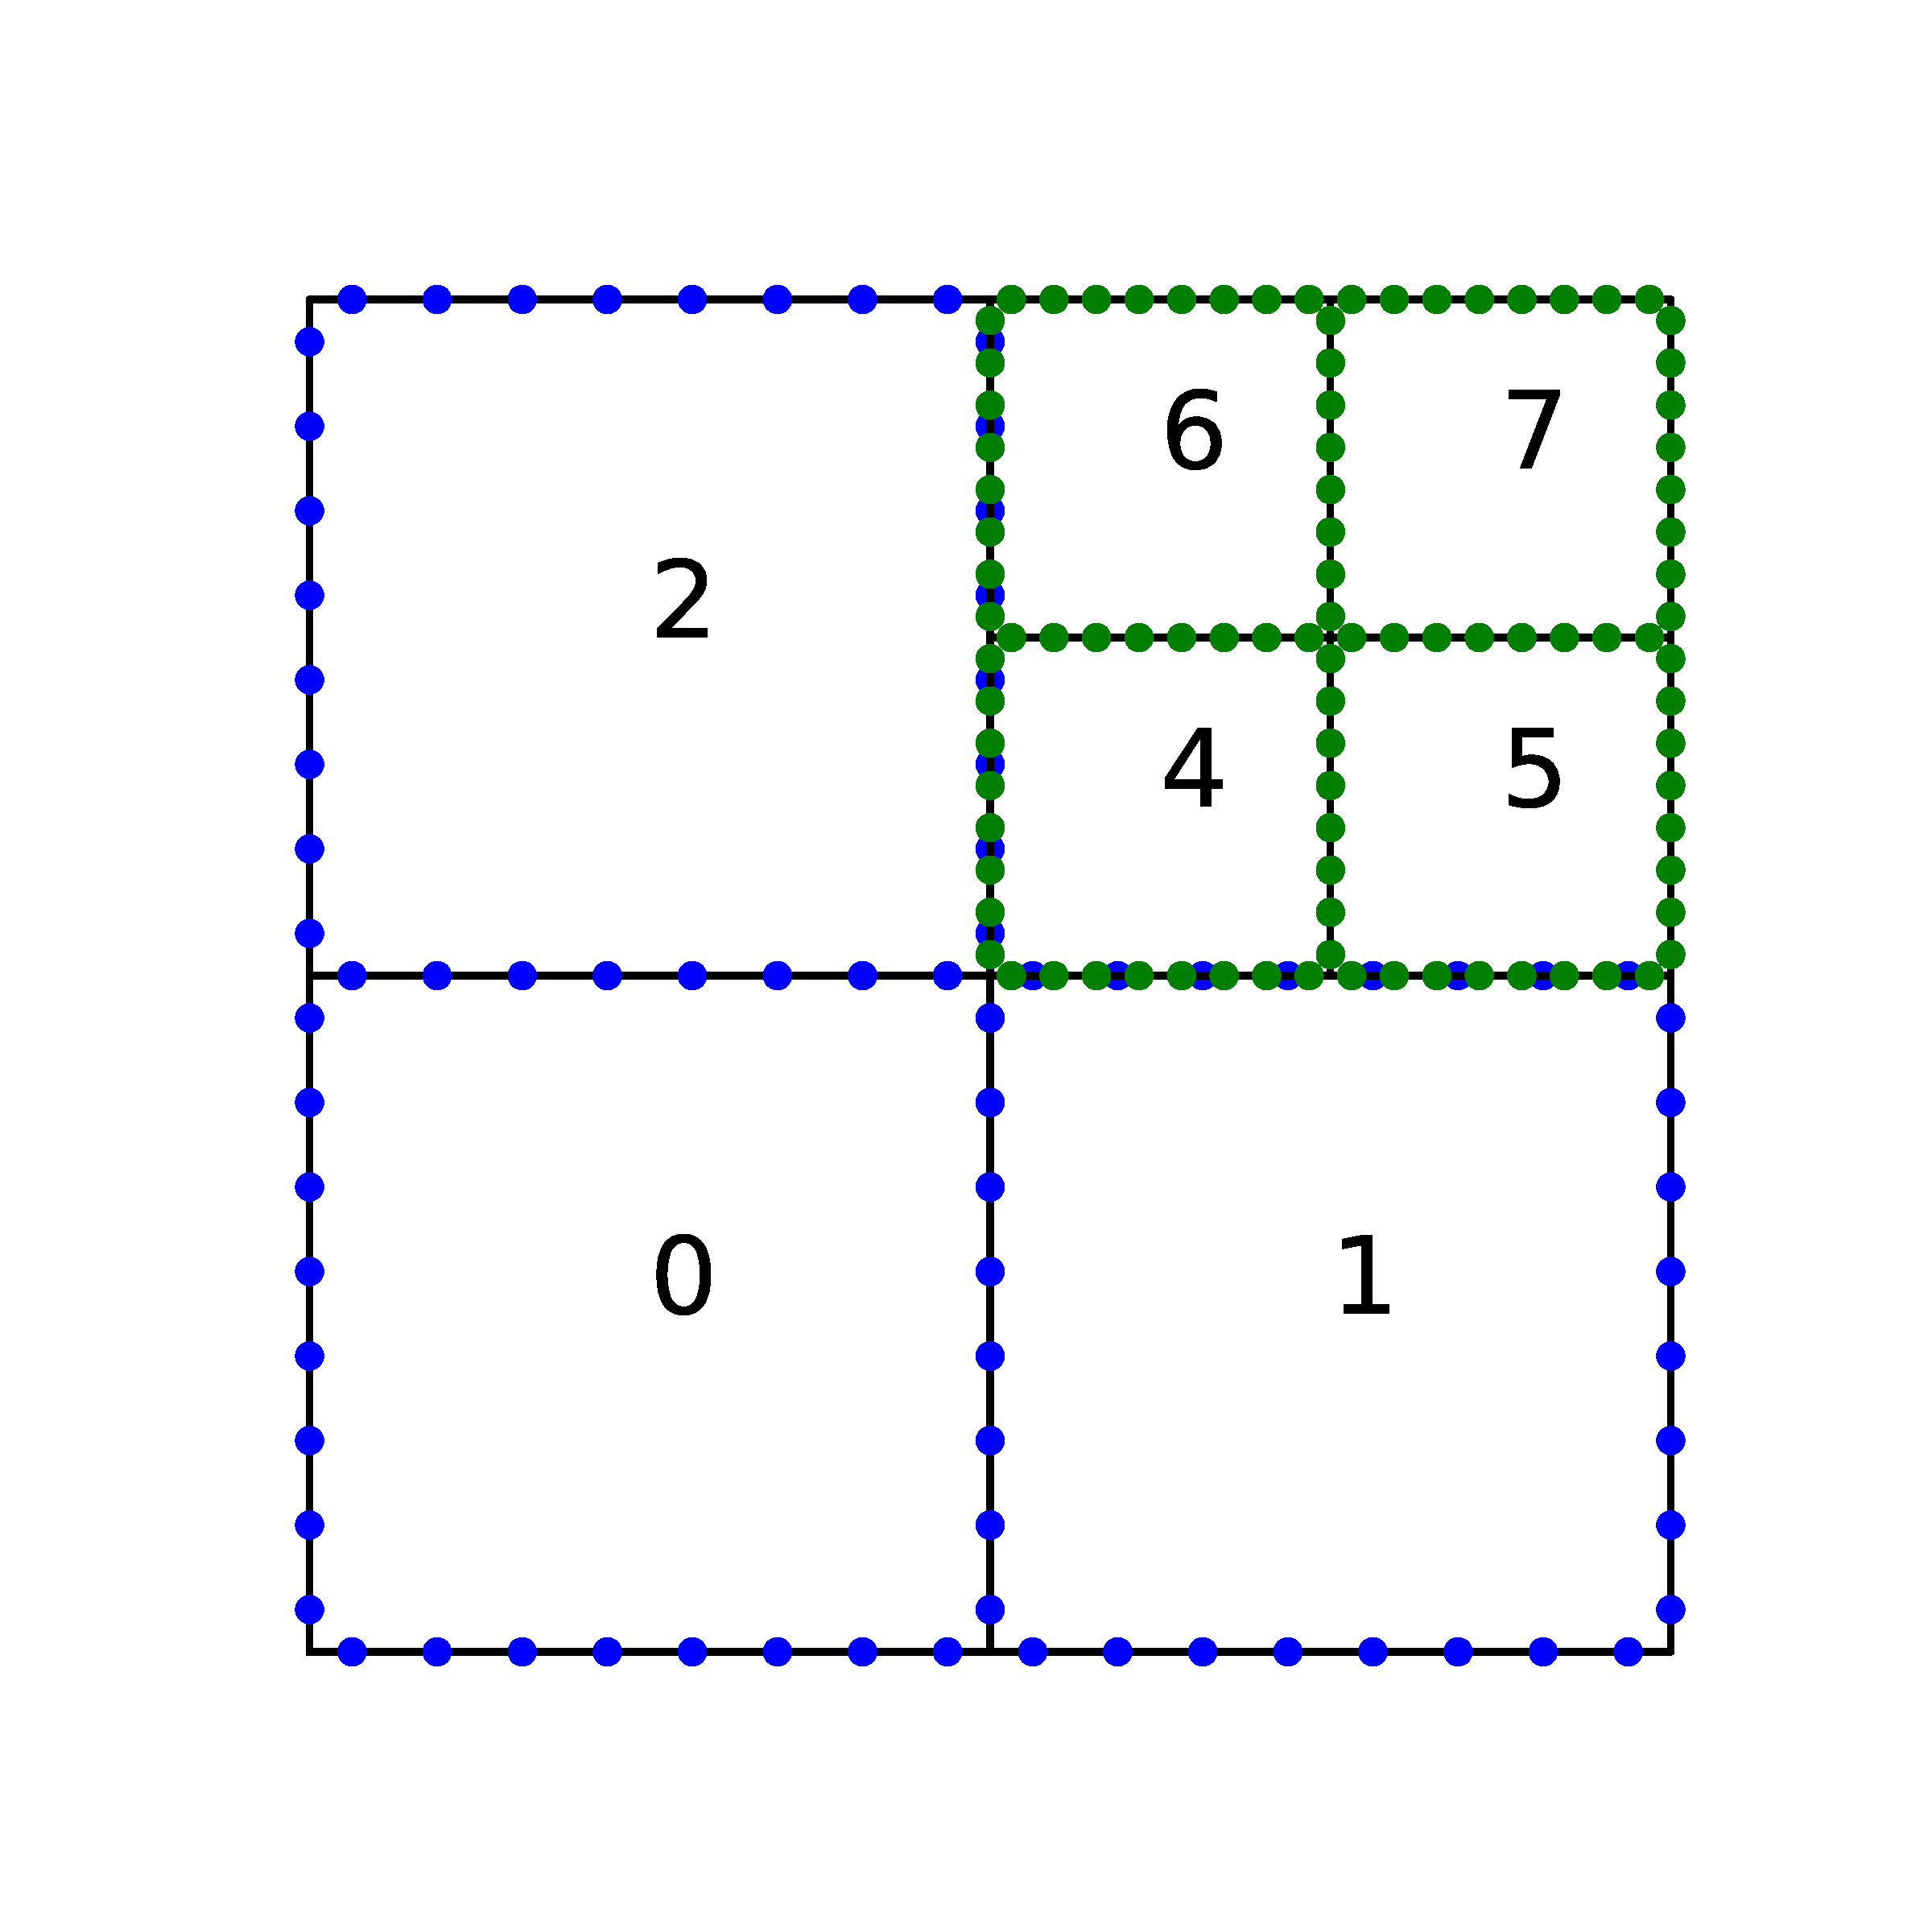
\includegraphics[width=\textwidth, clip=true, trim={100 150 100 150}]{figs/adaptive_merge1.pdf}
        \end{subfigure}
        &
        \begin{subfigure}[t]{0.3\textwidth}
            \centering
            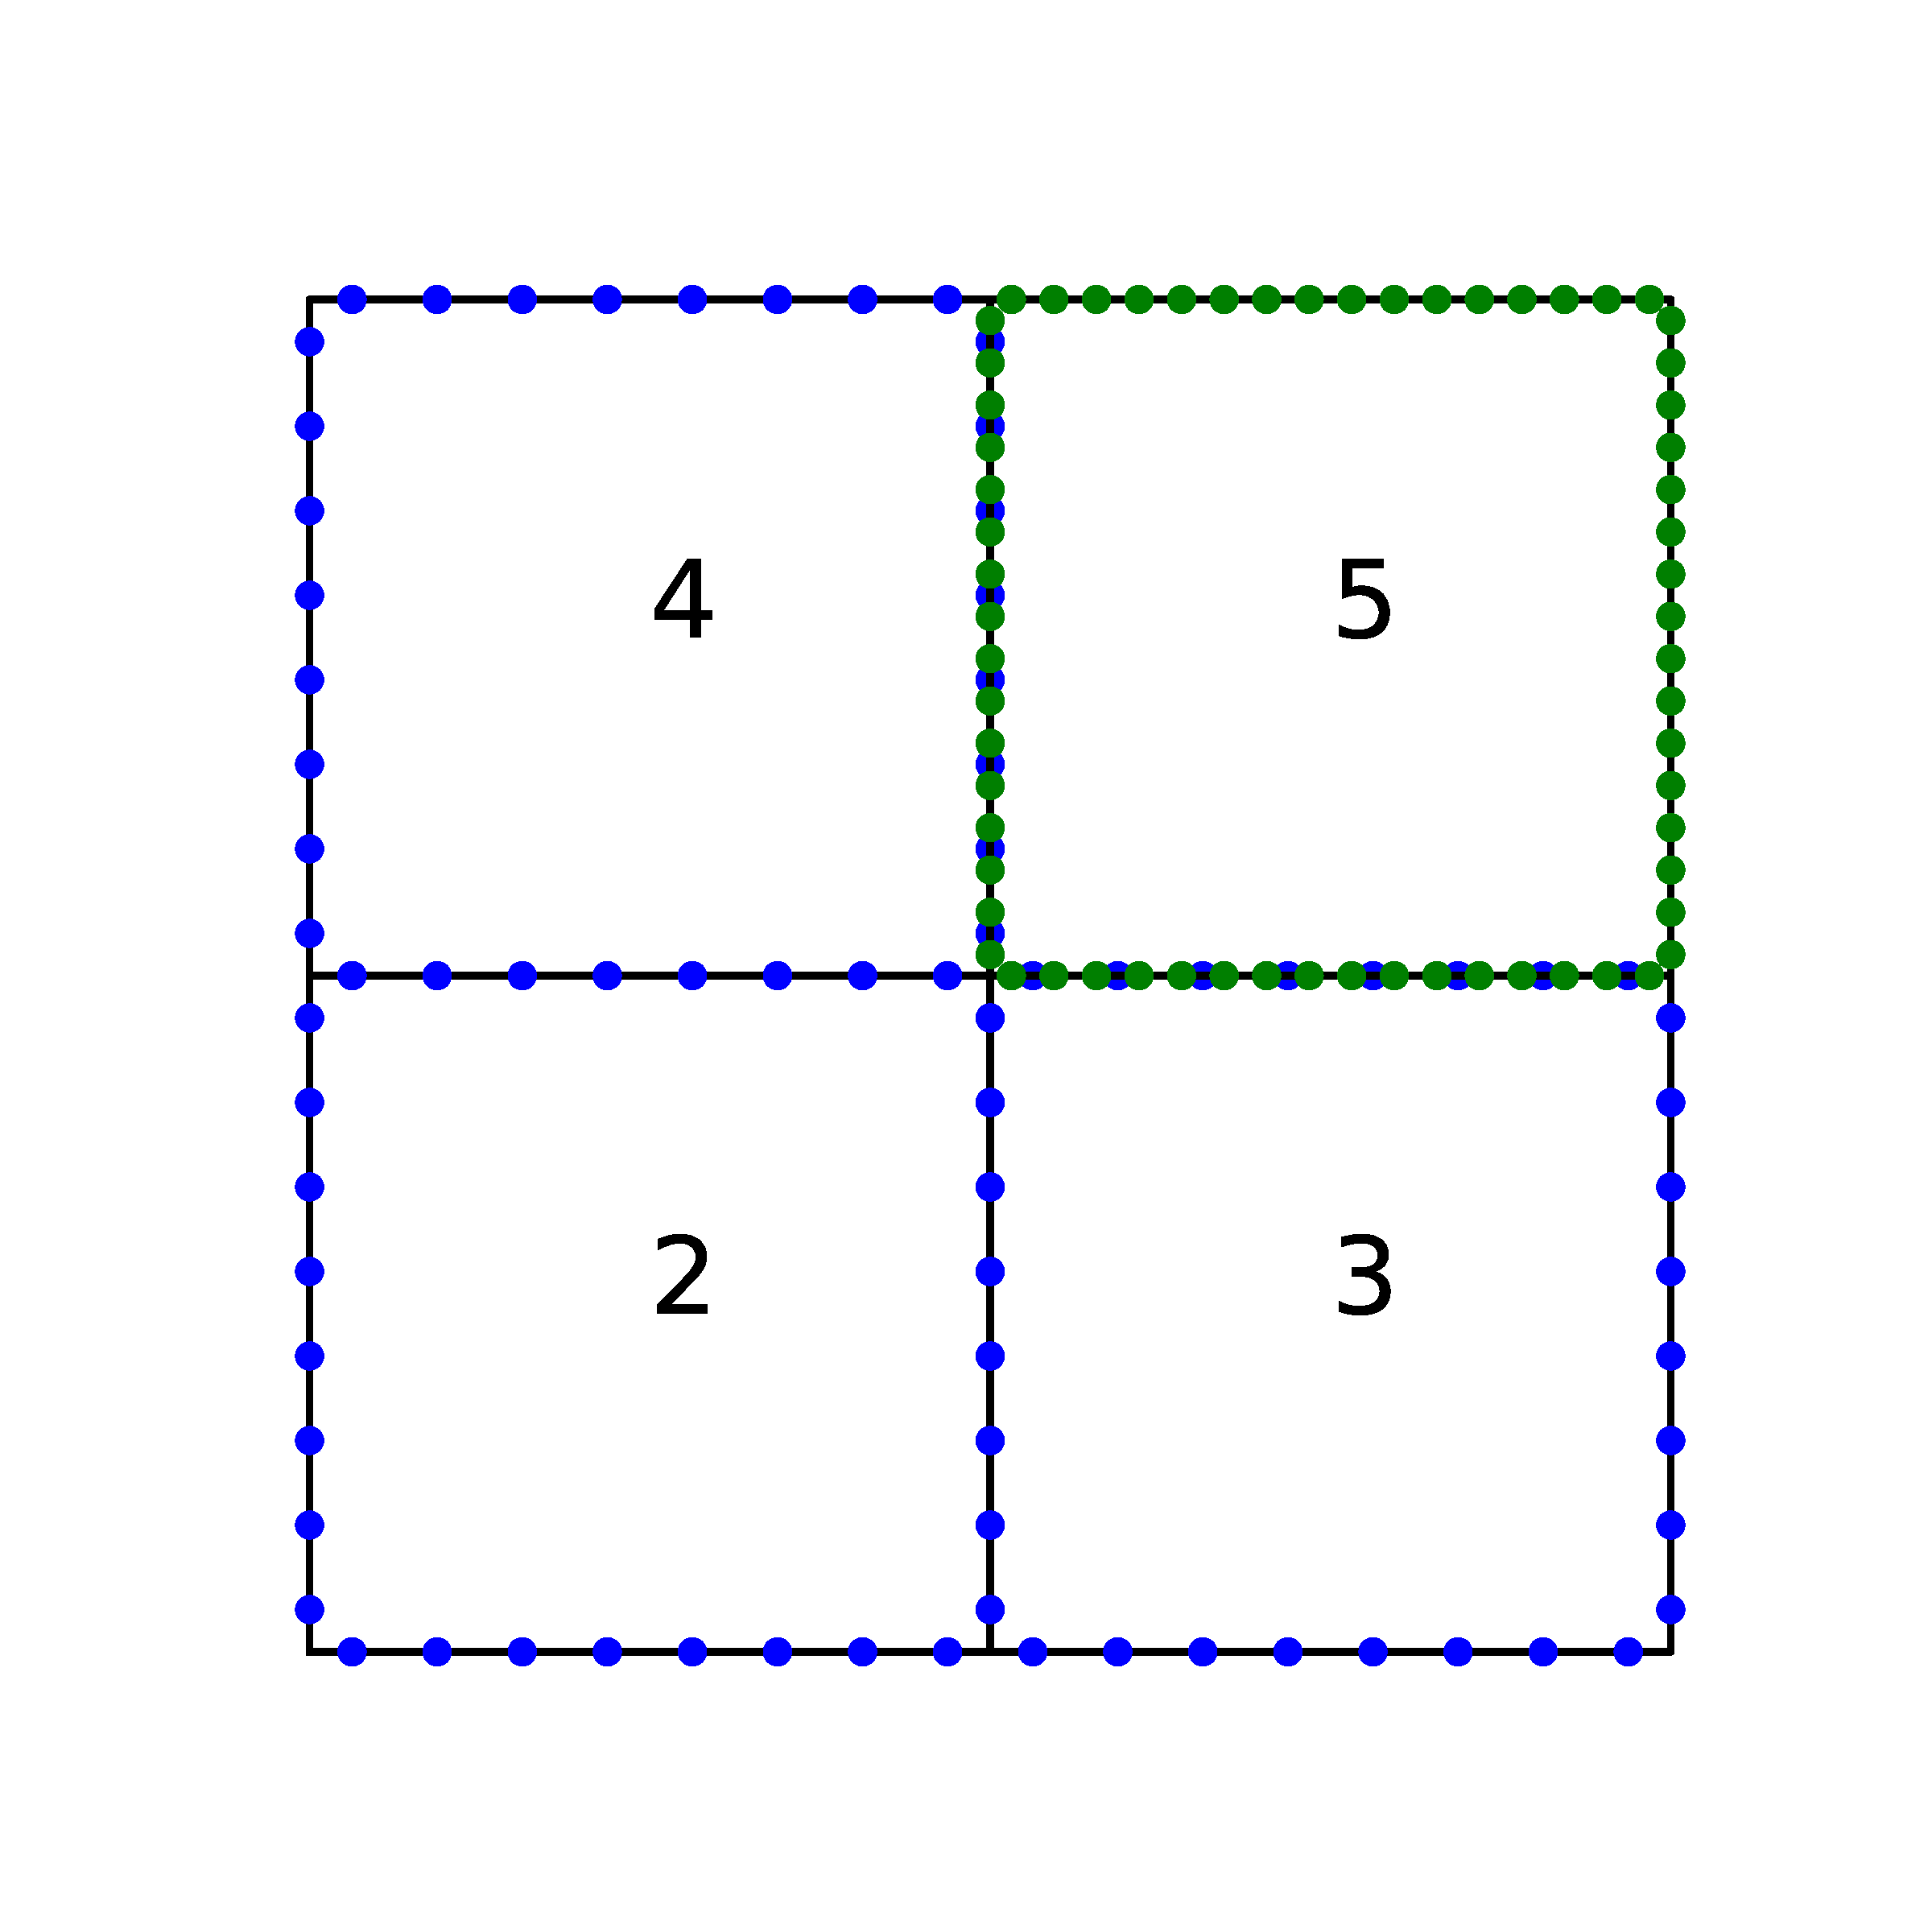
\includegraphics[width=\textwidth, clip=true, trim={100 150 100 150}]{figs/adaptive_merge2.pdf}
        \end{subfigure}
        &
        \begin{subfigure}[t]{0.3\textwidth}
            \centering
            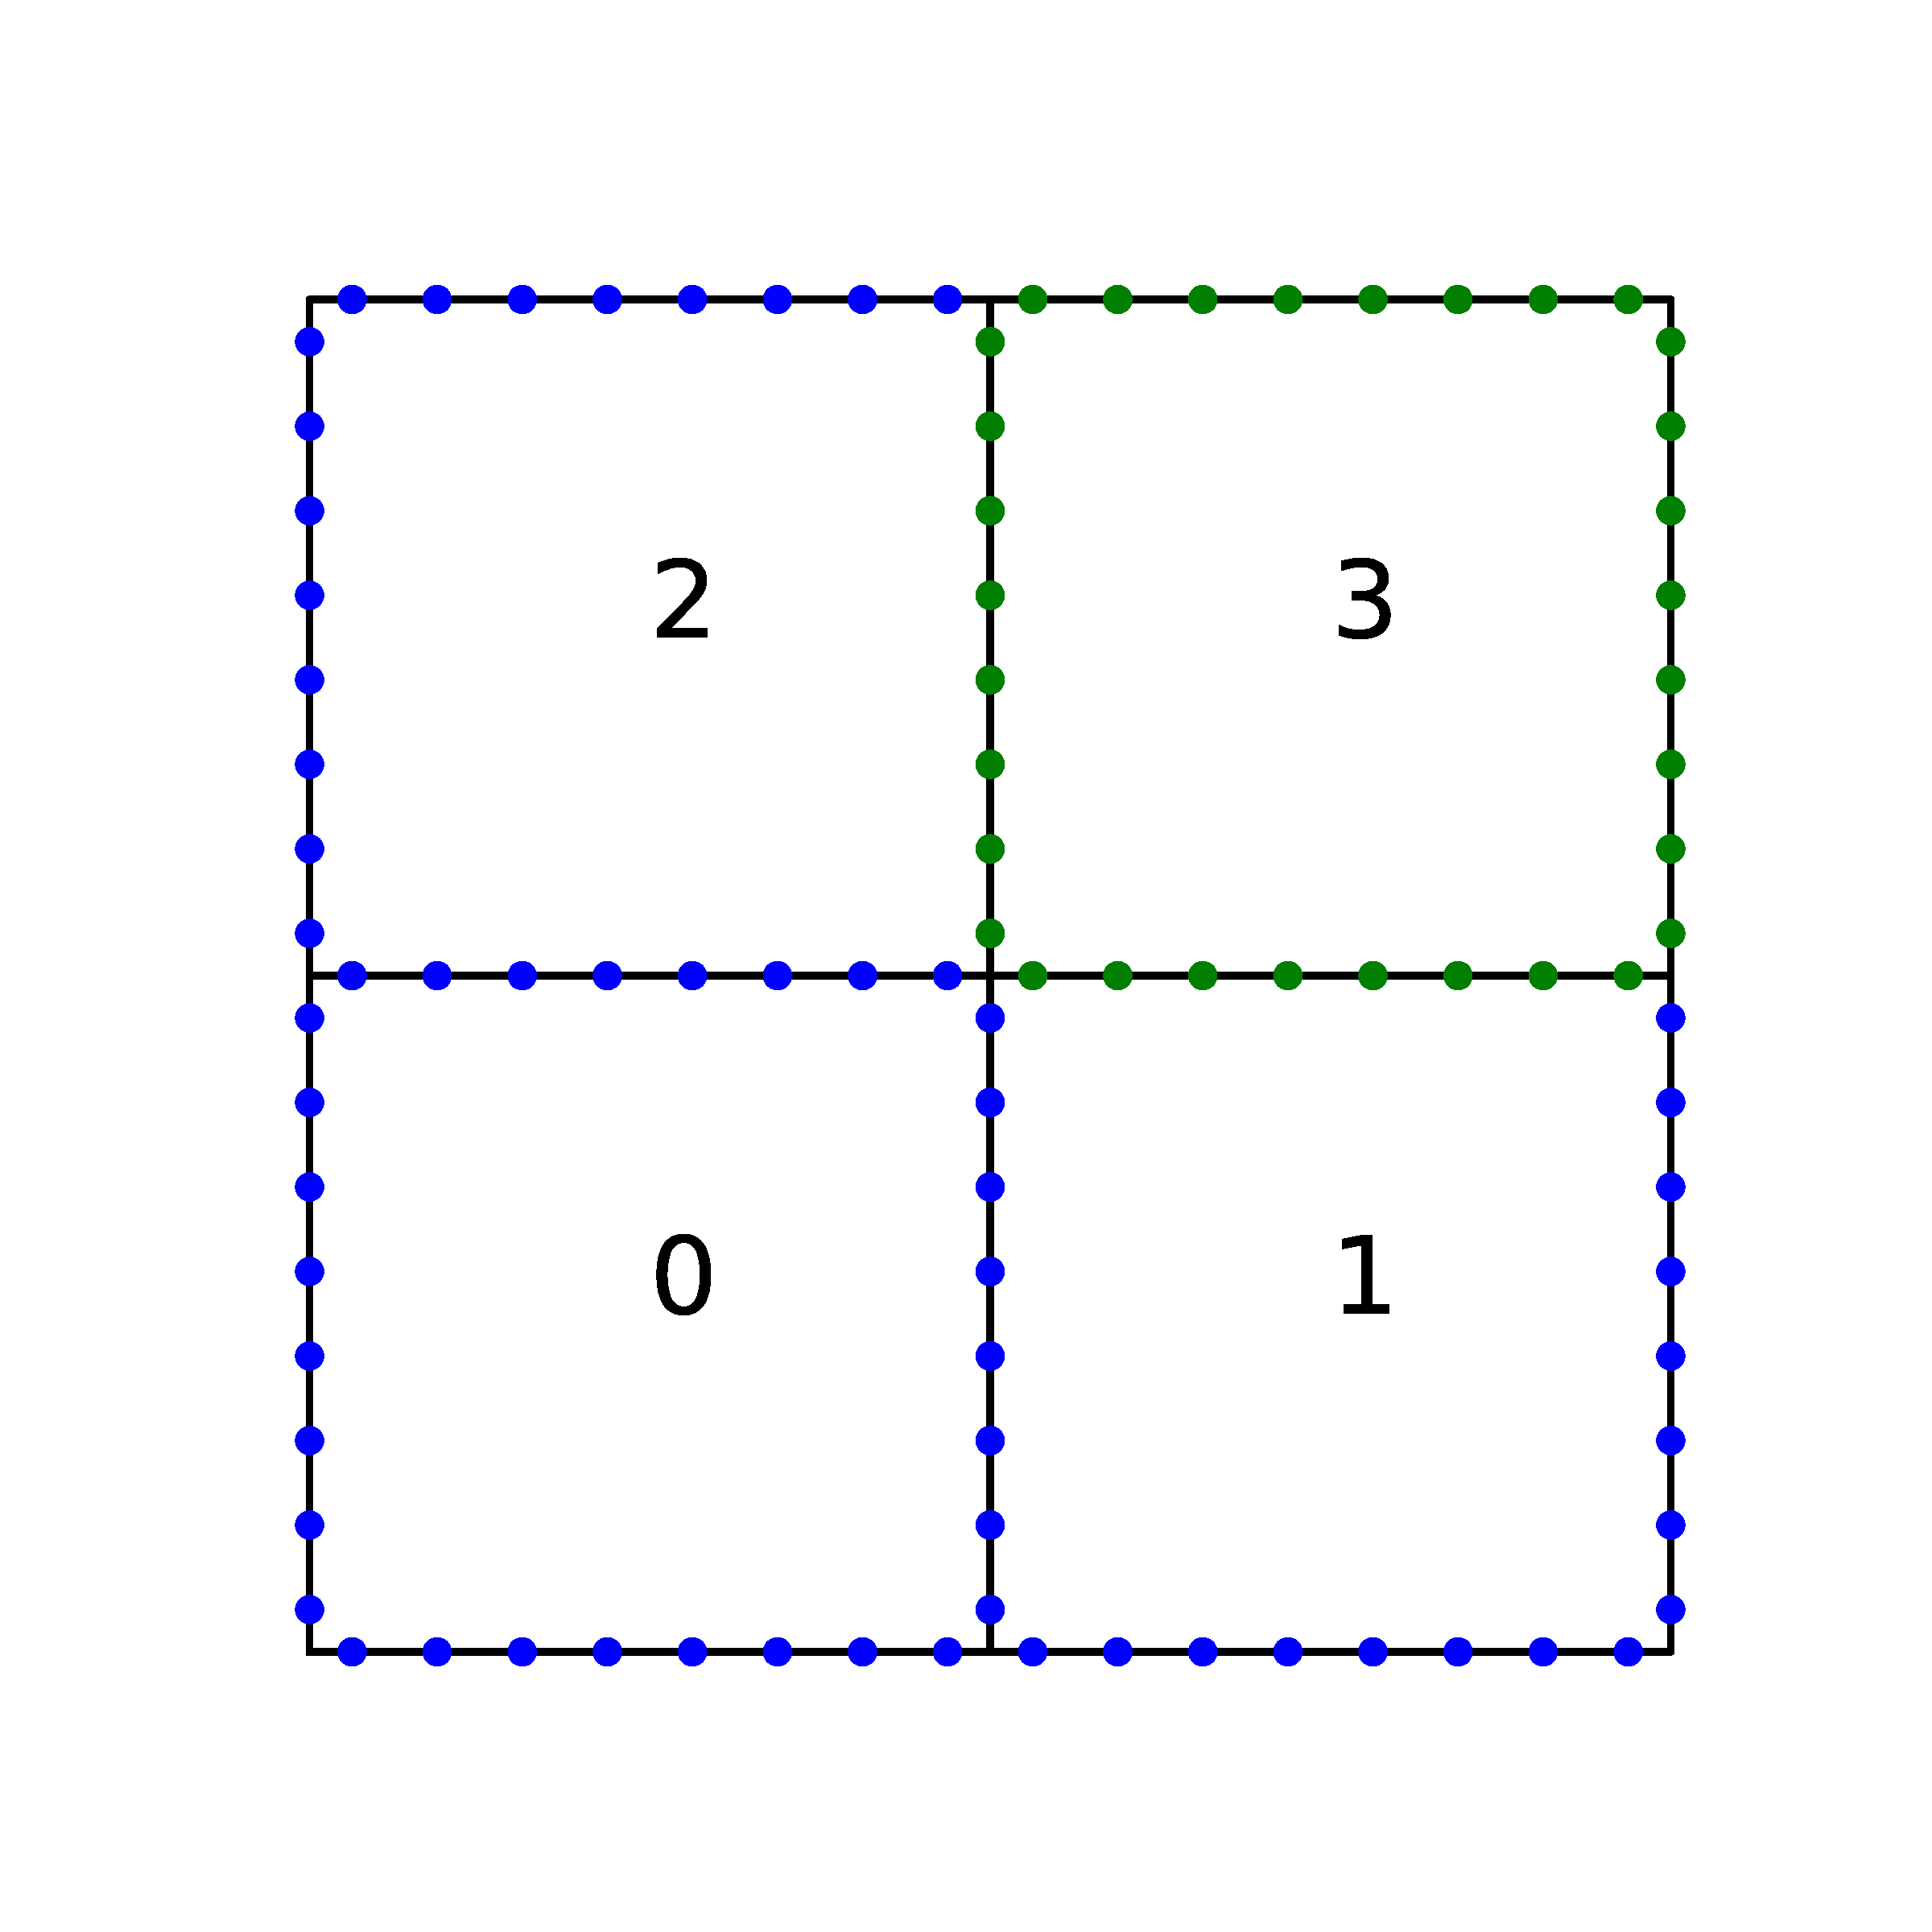
\includegraphics[width=\textwidth, clip=true, trim={100 150 100 150}]{figs/adaptive_merge3.pdf}
        \end{subfigure}
    \end{tabular}
    \caption{Example of a coarse-fine interface merge: (left) patches $6, 7, 8, \&\ 9$ will be merged and result in a coarse-fine interface, (middle) the data on patch 5 is averaged (coarsened), (right) merging $2, 3, 4, \&\ 5$ can continue as detailed in \refsec{sub:4-to-1merge}.}
    \label{fig:adaptive_merge}
\end{figure}

Prior to merging, we check each of the four children patches to be merged for a patch with data more fine than the other children. We do this by checking the size of the associated grid on that patch. Each patch that has data finer than the other siblings are tagged to be coarsened. Once tagged, the requisite data needed in the merge is coarsened via a block interpolation matrix.

For the build stage, only $\textbf{T}^{\tau}$ needs to be coarsened. For the upwards stage, $\textbf{h}^{\tau}$ needs to be coarsened. We form interpolation matrices $\textbf{L}_{2,1}$ and $\textbf{L}_{1,2}$ that map two sides to one or one side to two, respectively. As we employ a cell-centered grid, these matrices either average two data points to one, or interpolate one data point to two. Block diagonal versions of these are formed as
\begin{align}
    \textbf{L}_{2,1}^{B} &= \texttt{BlockDiag}(\textbf{L}_{2,1}, \textbf{L}_{2,1}, \textbf{L}_{2,1}, \textbf{L}_{2,1}) \\
    \textbf{L}_{1,2}^{B} &= \texttt{BlockDiag}(\textbf{L}_{1,2}, \textbf{L}_{1,2}, \textbf{L}_{1,2}, \textbf{L}_{1,2})
\end{align}
and coarsening $\textbf{T}$ and $\textbf{h}$ is done by matrix multiplication
\begin{align}
    \textbf{T}^{\tau'} &= \textbf{L}_{2,1}^{B} \textbf{T}^{\tau} \textbf{L}_{1,2}^{B} \\
    \textbf{h}^{\tau'} &= \textbf{L}_{2,1}^{B} \textbf{h}^{\tau}
\end{align}
where the prime indicates a coarsened version of that data.

A 1-to-4 split with a parent that has data that was coarsened during the 4-to-1 merge (for example, patch 5 from \reffig{fig:adaptive_merge}) needs to be un-coarsened. Traditionally, in the context of adaptive mesh refinement, this would be called refinement, but as the data was fine to start and coarsened during the merge, the data is un-coarsened. The requisite data that is un-coarsened is the boundary data, $\textbf{u}^{\tau}_{ext}$ in Equation \refeq{eq:S-times-u_ext}. This is done with the block diagonal interpolation matrices formed above:
\begin{align}
    \textbf{u}^{\tau}_{ext} = \textbf{L}_{1,2}^{B} \textbf{u}^{\tau'}_{ext}.
\end{align}

\subsection{Full Merging and Splitting Procedures}

Having discussed the merging and splitting procedures, as well as how to handle coarse-fine interfaces, we can now outline the algorithms that perform the 4-to-1 merge and the 1-to-4 split. They are laid out in Algorithms \ref{alg:build_merge}, \ref{alg:upwards_merge}, and \ref{alg:solve_split}.

\begin{algorithm}[H]
    \caption{\texttt{Merge4To1} Function}
    \begin{algorithmic}[0]
        \Require Patch data: $\textbf{T}^{\alpha}$, $\textbf{T}^{\beta}$, $\textbf{T}^{\gamma}$, $\textbf{T}^{\omega}$
        \For{$i = \alpha, \beta, \gamma, \omega$} \Comment{Iterate over children and check for coarse-fine interface}
            \State \texttt{tag} = \texttt{TagForCoarsening}(i)
            \If{\texttt{tag}}
                \State Coarsen: $\textbf{T}^{i} = \textbf{L}_{2,1} \textbf{T}^{i} \textbf{L}_{1,2}$
            \EndIf
        \EndFor
        \State Create external index sets: $\textbf{I}_{\alpha \tau}, \textbf{I}_{\beta \tau}, \textbf{I}_{\gamma \tau}, \textbf{I}_{\omega \tau}$ \Comment{See \reffig{fig:merged_index_sets}}
        \State Create internal index sets: $\textbf{I}_{\alpha \gamma}, \textbf{I}_{\beta \omega}, \textbf{I}_{\alpha \beta}, \textbf{I}_{\gamma \omega}$ \Comment{See \reffig{fig:merged_index_sets}}
        \State Compute matrices $\textbf{A}, \textbf{B}, \textbf{C}, \textbf{D}$ according to Equations \refeq{eq:matrix_AB} and \refeq{eq:matrix_CD}. 
        \State \Comment{Compute merged data}
        \State Compute $\textbf{X}^{\tau} = \textbf{D}^{-1}$
        \State Compute $\textbf{S}^{\tau} = \textbf{D}^{-1} \textbf{C}$
        \State Compute $\textbf{T}^{\tau} = \textbf{A} - \textbf{B} \textbf{D}^{-1} \textbf{C}$
    \end{algorithmic}
    \label{alg:build_merge}
\end{algorithm}

\begin{algorithm}[H]
    \caption{\texttt{Upwards4To1} Function}
    \begin{algorithmic}[0]
        \Require Patch data: $\textbf{T}^{\alpha}$, $\textbf{T}^{\beta}$, $\textbf{T}^{\gamma}$, $\textbf{T}^{\omega}$, $\textbf{h}^{\alpha}$, $\textbf{h}^{\beta}$, $\textbf{h}^{\gamma}$, $\textbf{h}^{\omega}$
        \For{$i = \alpha, \beta, \gamma, \omega$} \Comment{Iterate over children and check for coarse-fine interface}
            \State \texttt{tag} = \texttt{TagForCoarsening}(i)
            \If{\texttt{tag}}
                \State Coarsen: $\textbf{h}^{i} = \textbf{L}_{2,1} \textbf{h}^{i}$
            \EndIf
        \EndFor
        \State Create external index sets: $\textbf{I}_{\alpha \tau}, \textbf{I}_{\beta \tau}, \textbf{I}_{\gamma \tau}, \textbf{I}_{\omega \tau}$ \Comment{See \reffig{fig:quadtree_indexing}}
        \State Create internal index sets: $\textbf{I}_{\alpha \gamma}, \textbf{I}_{\beta \omega}, \textbf{I}_{\alpha \beta}, \textbf{I}_{\gamma \omega}$ \Comment{See \reffig{fig:quadtree_indexing}}
        \State Compute matrices $\textbf{B}, \textbf{D}$ according to Equations \refeq{eq:matrix_AB}, \refeq{eq:matrix_CD}
        \State Compute $\textbf{h}_{diff}$ according to Equation \refeq{eq:h_diff} \Comment{Flux data across interface}
        \State \Comment{Compute merged data}
        \State Compute $\textbf{X}^{\tau} = \textbf{D}^{-1}$
        \State Compute $\textbf{w}^{\tau} = \textbf{X}^{\tau} \textbf{h}_{diff}$
        \State Compute update $\textbf{h}^{\tau} = \textbf{h}^{\tau} + \textbf{B} \textbf{w}^{\tau}$
    \end{algorithmic}
    \label{alg:upwards_merge}
\end{algorithm}

\begin{algorithm}[H]
    \caption{\texttt{Split1To4} Function}
    \begin{algorithmic}[0]
        \Require Patch data: $\textbf{S}^{\tau}$, $\textbf{g}^{\tau} = \textbf{u}^{\tau}_{ext}$
        \State \texttt{tag} = \texttt{TagForUncoarsening}($\tau$) \Comment{Check for coarsened patch}
        \If{\texttt{tag}}
            \State Uncoarsen: $\textbf{g}^{\tau} = \textbf{L}_{1,2} \textbf{g}^{\tau}$ \Comment{Interpolate coarse to fine on boundary}
        \EndIf
        \State Create external index sets: $\textbf{I}_{\alpha \tau}, \textbf{I}_{\beta \tau}, \textbf{I}_{\gamma \tau}, \textbf{I}_{\omega \tau}$ \Comment{See \reffig{fig:quadtree_indexing}}
        \State Create internal index sets: $\textbf{I}_{\alpha \gamma}, \textbf{I}_{\beta \omega}, \textbf{I}_{\alpha \beta}, \textbf{I}_{\gamma \omega}$ \Comment{See \reffig{fig:quadtree_indexing}}
        \State Compute $\textbf{u}_{int} = \textbf{S}^{\tau} \textbf{u}^{\tau}_{ext} + \textbf{w}^{\tau}$ \Comment{Apply solution operator}
        \State Partition $\textbf{u}_{int}$ into $\textbf{u}_{\alpha \gamma}, \textbf{u}_{\beta \omega}, \textbf{u}_{\alpha \beta}, \textbf{u}_{\gamma \omega}$
        \State \Comment{Reorder interface data to children exterior data}
        \State Create $\textbf{u}^{\alpha}_{ext}, \textbf{u}^{\beta}_{ext}, \textbf{u}^{\gamma}_{ext}, \textbf{u}^{\omega}_{ext}$ according to Equations \refeq{eq:u_ext_alpha}, \refeq{eq:u_ext_beta}, \refeq{eq:u_ext_gamma}, \refeq{eq:u_ext_omega}
    \end{algorithmic}
    \label{alg:solve_split}
\end{algorithm}

\subsection{Comparison Between 4-to-1 Merging and 2-to-1 Merging}
\label{sub:comparison_between_4t1_and2t1_merging}

Here, we compare the performance and storage requirements for the 4-to-1 merge outlined in this paper against the 2-to-1 merge presented in \citep{gillman2014direct}. In \citep{gillman2014direct}, merging is done between two neighboring patches. To merge a family of four patches, one must do two vertical merges (merge two neighboring patches that lie next to each other in the y-direction) and then one horizontal merge (merge two ``tall-skinny'' patches that lie next to each other in the x-direction). Thus, computing and storing $\textbf{T}^{\tau}$ and $\textbf{S}^{\tau}$ requires three, 2-to-1 merges; two vertical merges and one horizontal merge.

For both approaches, we assume that a patch has $M$ points per side, resulting in $M^2$ points per patch. We will compare the floating point operations per second (FLOPS), or FLOP count, as well as the memory needed to store the computed matrices. The merge process is seen as an elimination of the points on the interface of neighboring patches. For the 2-to-1 vertical merge, computing $\textbf{S}$ requires $M^3$ FLOPS as a linear solve is necessary, and computing $\textbf{T}$ requires $36M^3$ FLOPS. Storing $\textbf{S}$ and $\textbf{T}$ requires $6M^2$ and $36M^2$ numbers, respectively. For the 2-to-1 horizontal merge, computing $\textbf{S}$ requires $8M^3$ FLOPS and computing $\textbf{T}$ requires $128M^3$ FLOPS. Storing $\textbf{S}$ and $\textbf{T}$ requires $16M^2$ and $64M^2$ numbers, respectively. Thus, for a full 4-to-1 merge via two vertical merges and one horizontal merge, the total FLOP count is $210M^3$, with storage for $164M^2$ numbers. For the 4-to-1 merge, computing $\textbf{S}$ requires $64M^3$ FLOPS and computing $\textbf{T}$ requires $256M^3$ FLOPS. Storing $\textbf{S}$ and $\textbf{T}$ requires $32M^2$ and $64M^2$ numbers, respectively. Thus, for a 4-to-1 merge outlined in this paper, the total FLOP count is $320M^3$, with storage for $96M^2$ numbers. As can be seen, the method presented herein has slightly higher FLOP count than the one outlined in \citep{gillman2014direct}, requiring slightly less memory to store the computed matrices. As direct methods are often memory heavy, this is a non-trivial difference.